\documentclass{article}
\usepackage[utf8]{inputenc}
\usepackage{titling}
\usepackage{graphicx}
\usepackage{ragged2e}
\usepackage{float}

\title{SBS - TP4}
\author{Gonçalo Almeida (A84610)}
\date{Novembro 2020}

\begin{document}

\begin{figure}[t]
    \centering
    
\includegraphics[scale=0.4]{Images/MIEI_logo.png}
\end{figure}

\title{
    \textbf{
        Universidade do Minho \\
        Departamento de Informática \\
        \vspace{1.5cm}
        Sistemas Baseados em Similaridade \\
        \vspace{1cm}
        Trabalho Prático Individual 4}
        \vspace{4cm}}

\maketitle

\clearpage

\section{Tarefa 1}

\subsection{Carregar, no Knime, o dataset descarregado e explorar os dados;}

\begin{figure}[H]
    \centering
    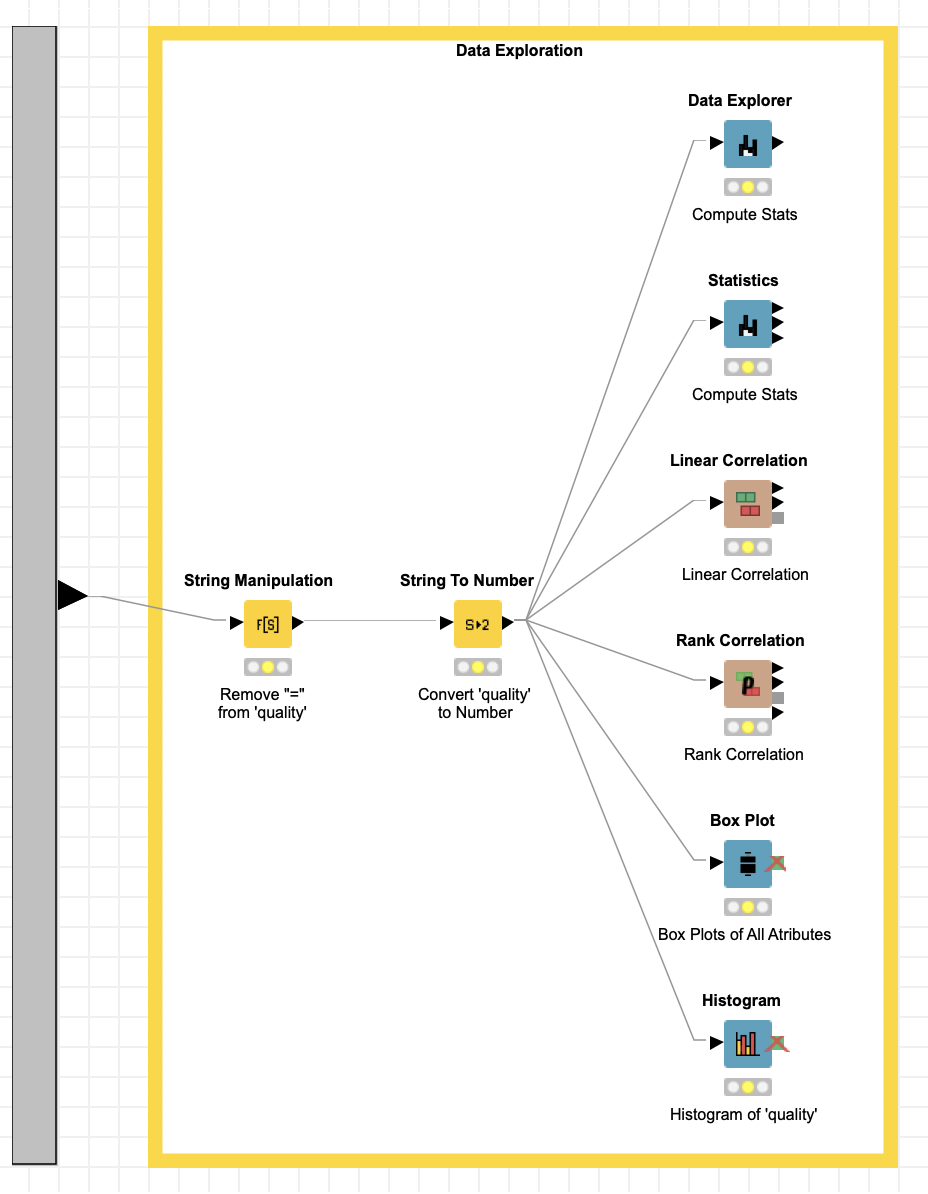
\includegraphics[scale=0.6]{Images/T1.png}
    \caption{Metanodo Data Exploration}
\end{figure}

\clearpage

\section{Tarefa 2}

\subsection{Tratar os dados, i.e.:}

\subsubsection{Fazer cast do atributo “quality” para inteiro;}

\begin{figure}[H]
    \centering
    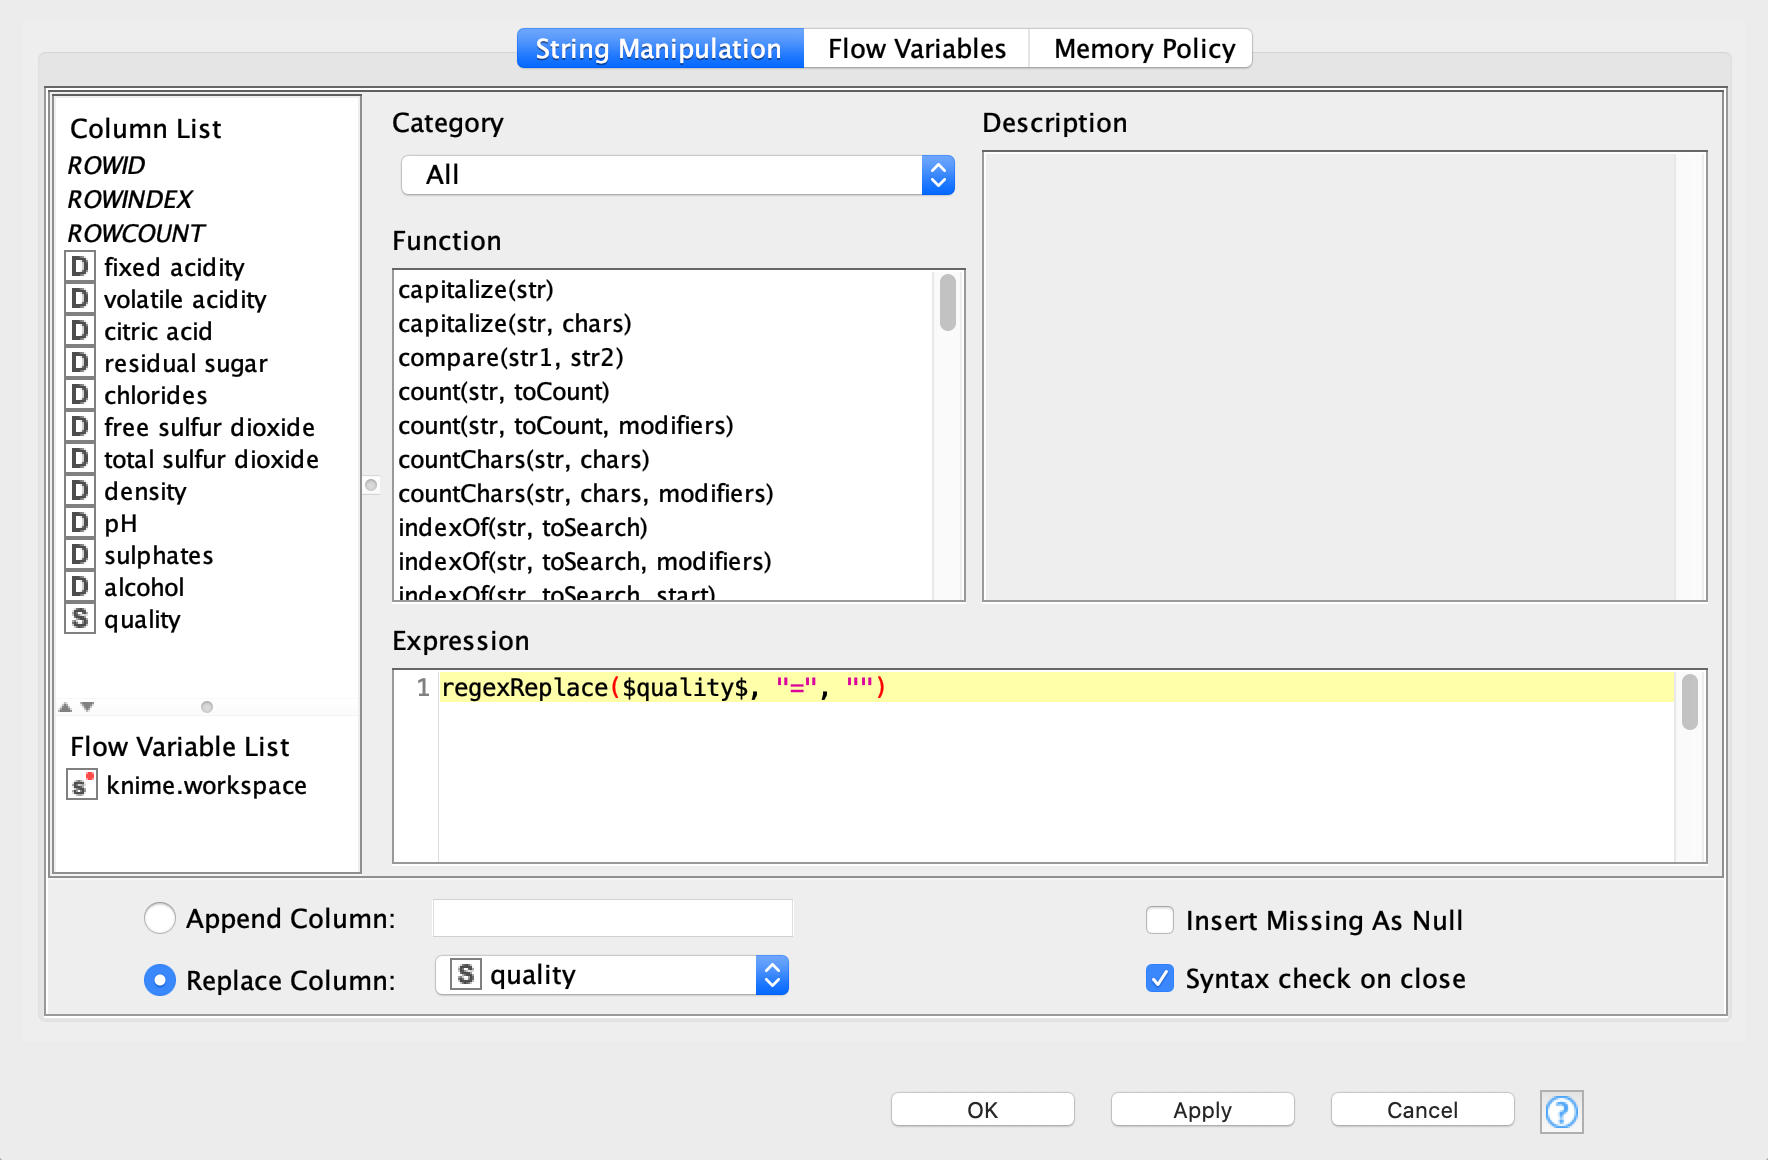
\includegraphics[scale=0.3]{Images/T2_a1.png}
    \caption{Remover o caracter "=" do atributo 'quality'}
\end{figure}

\begin{figure}[H]
    \centering
    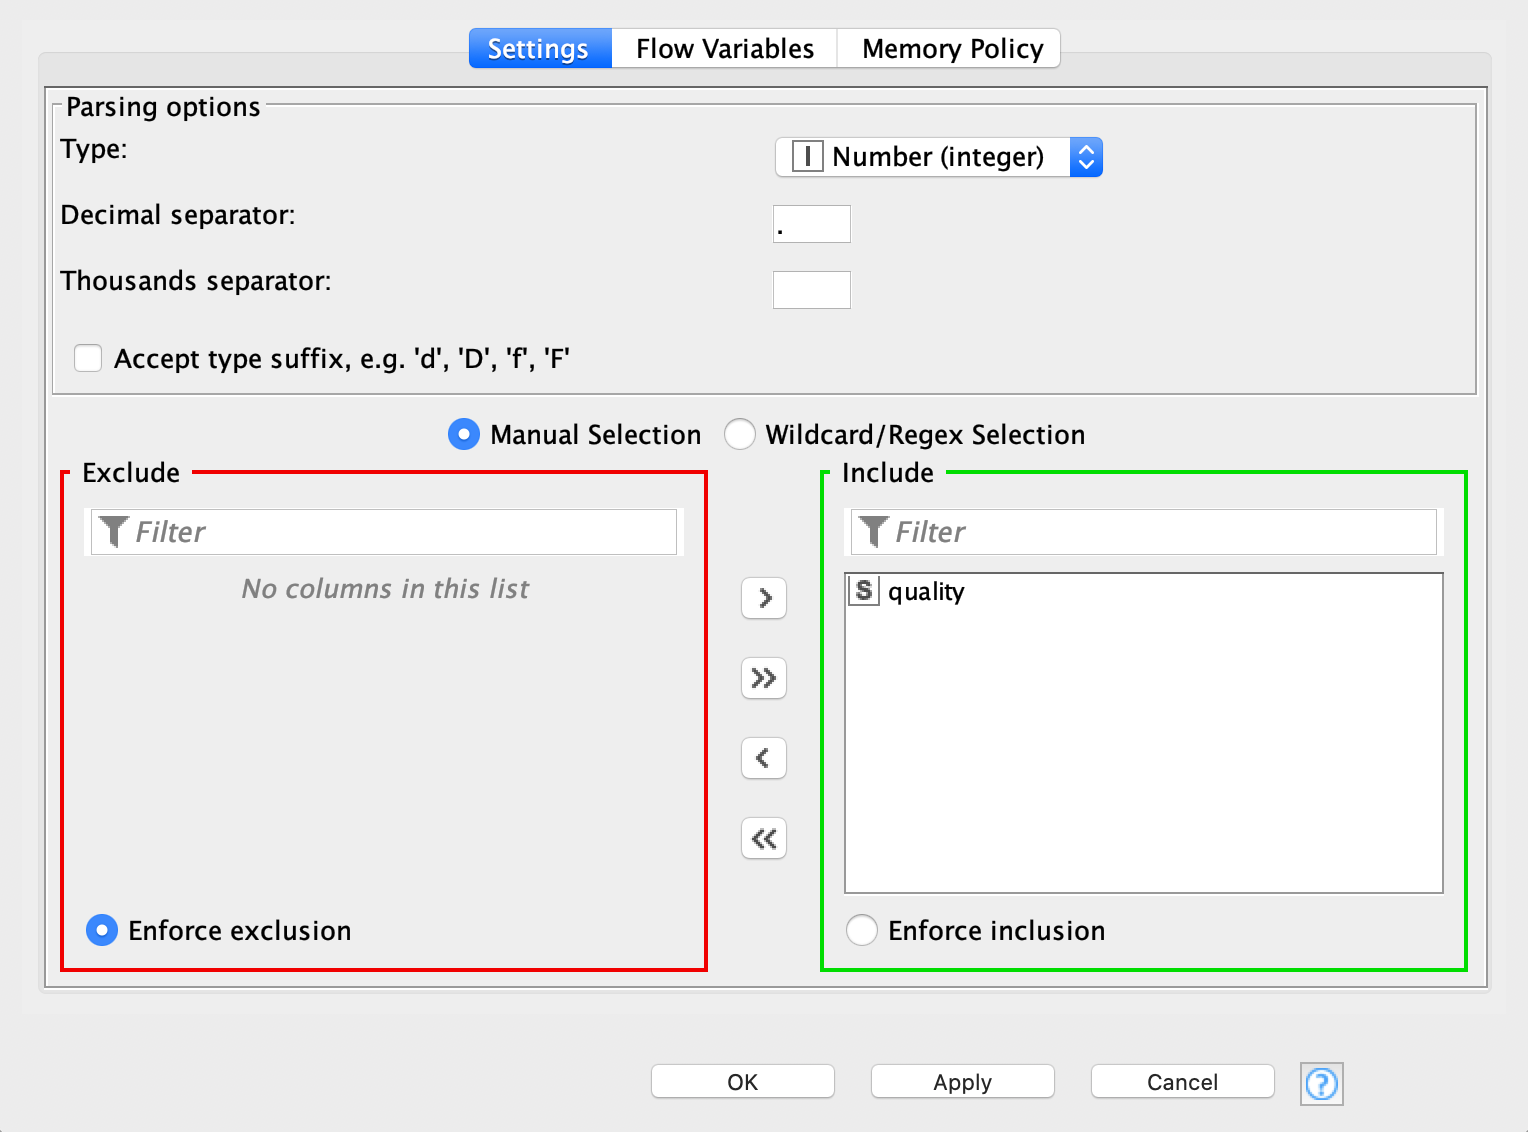
\includegraphics[scale=0.3]{Images/T2_a2.png}
    \caption{Cast do atributo 'quality'}
\end{figure}

\subsubsection{Normalizar todos os atributos numéricos utilizando a transformação linear Min- max de forma a produzir um input normalizado entre 0 e 1;}

\begin{figure}[H]
    \centering
    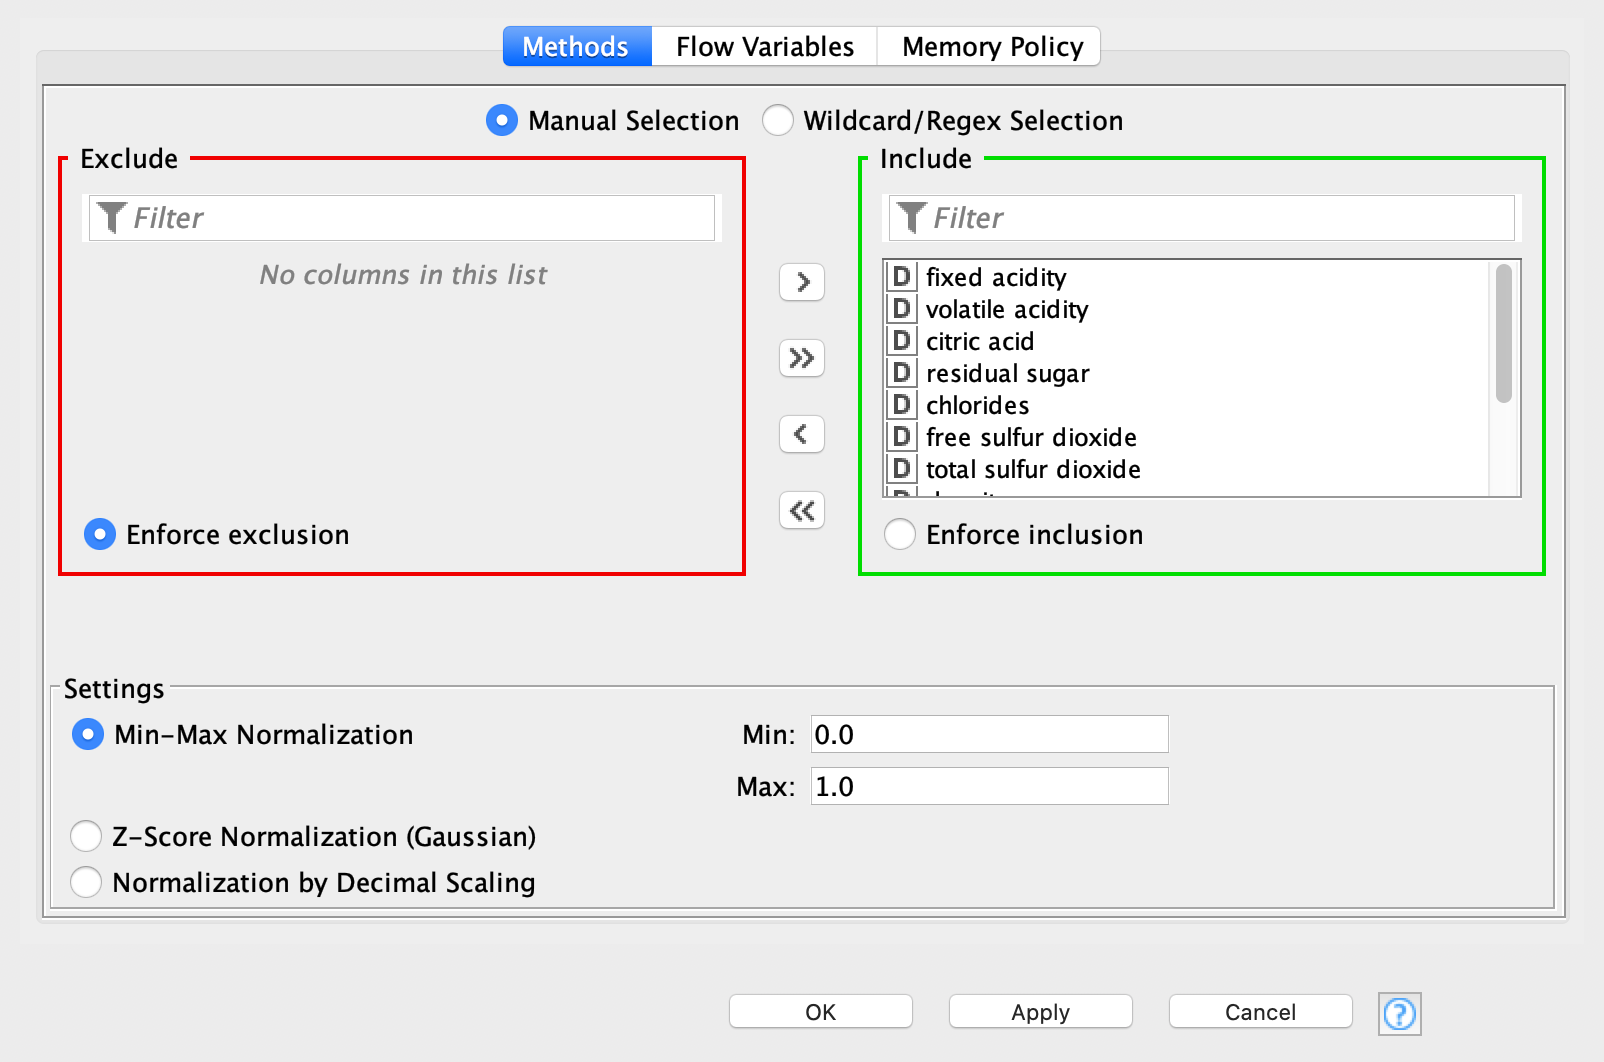
\includegraphics[scale=0.3]{Images/T2_b.png}
    \caption{Normalização dos atributos numéricos}
\end{figure}

\subsubsection{Criar 4 bins de igual frequência para a feature “citric acid”, substituindo a feature original;}

\begin{figure}[H]
    \centering
    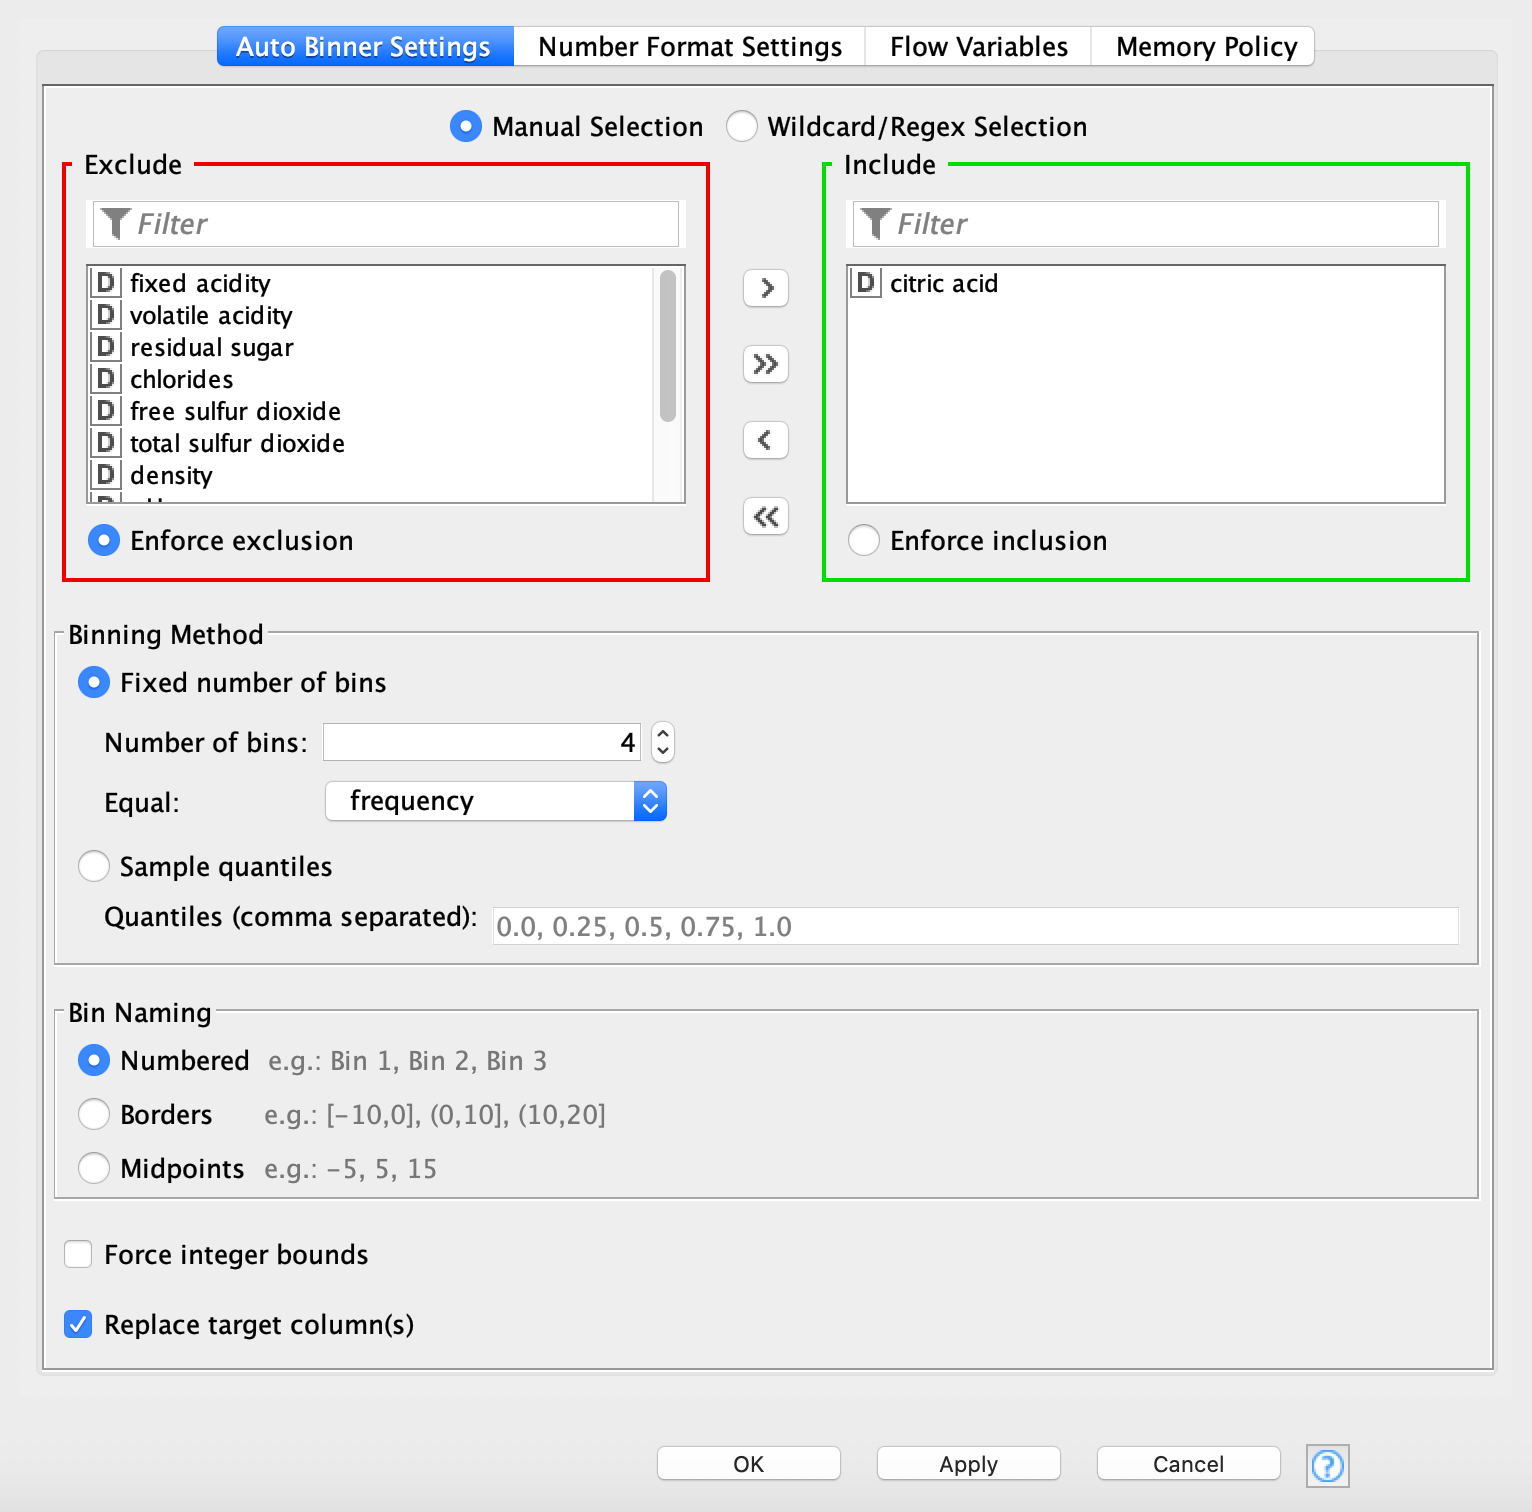
\includegraphics[scale=0.3]{Images/T2_c.png}
    \caption{Normalização dos atributos numéricos}
\end{figure}

\subsubsection{Renomear cada bin de forma a que o primeiro corresponda a Low, o segundo a Medium, o terceiro a High e o quarto a Very High.}

\begin{figure}[H]
    \centering
    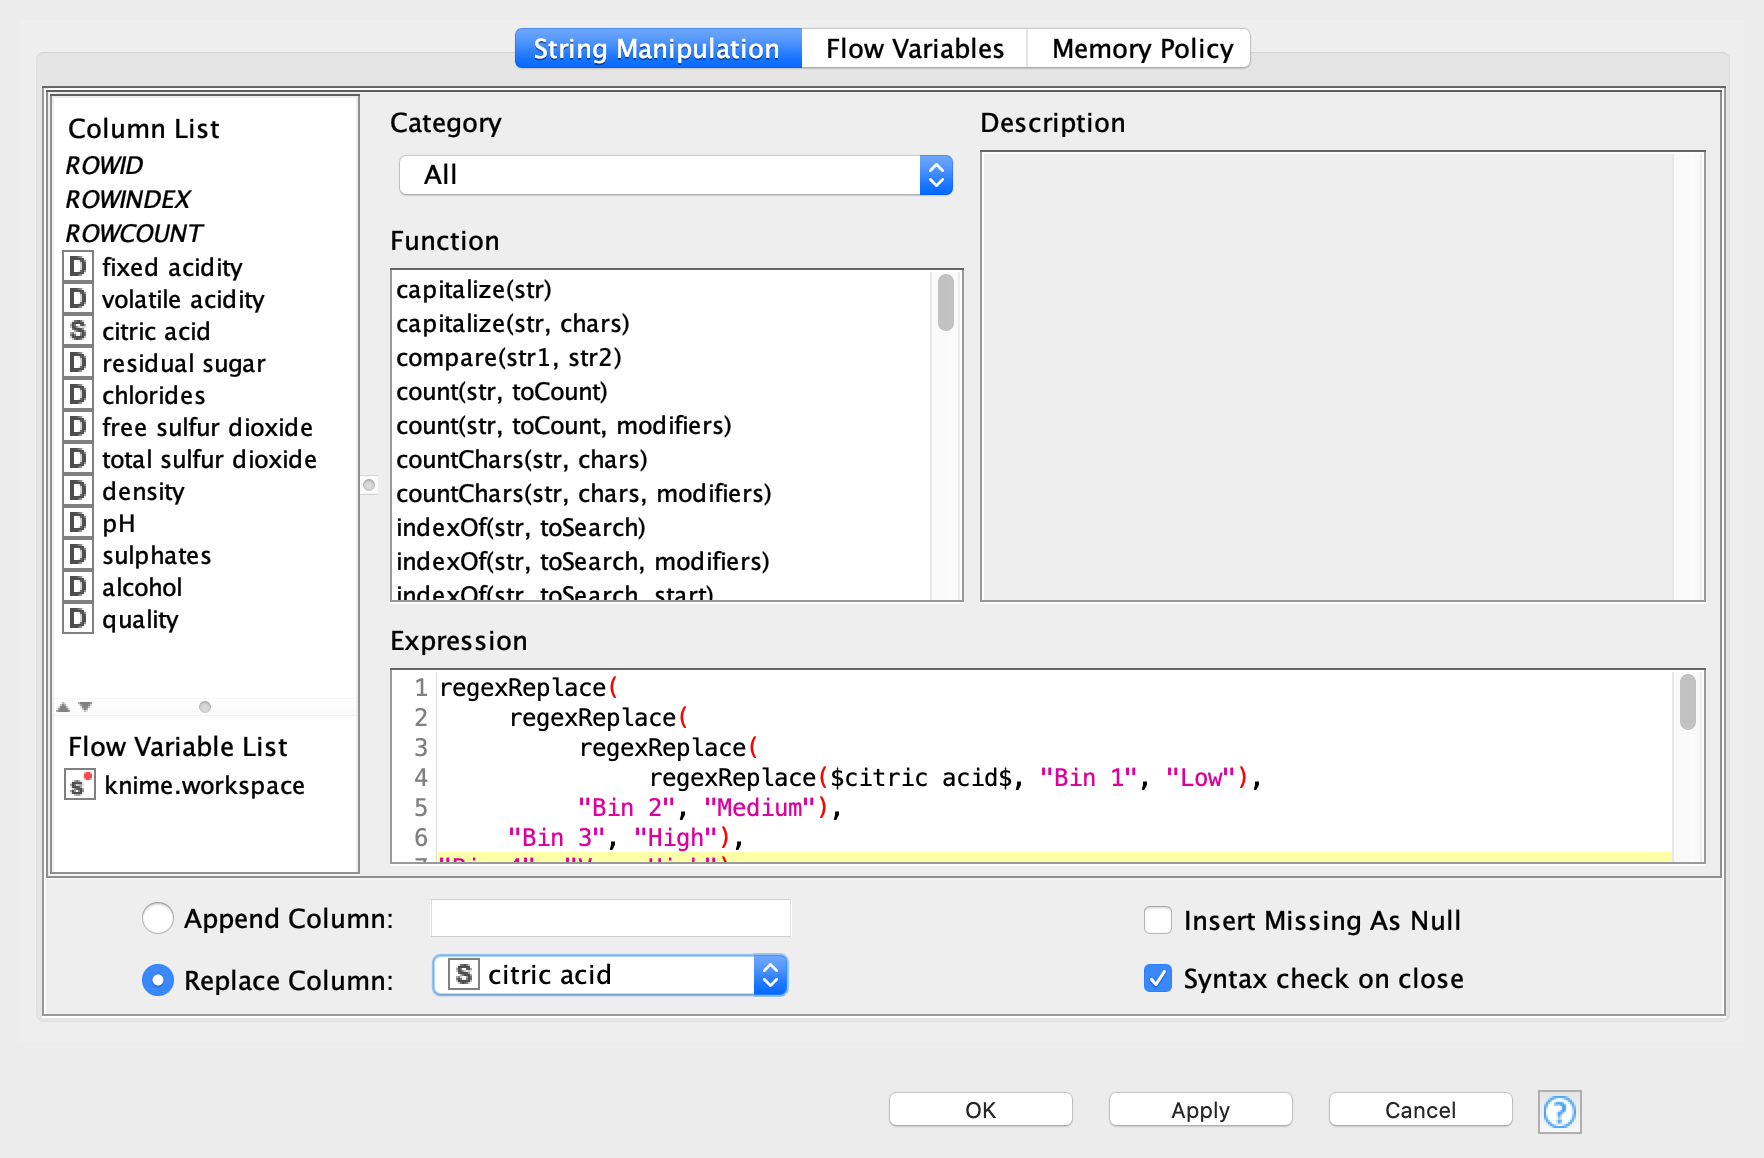
\includegraphics[scale=0.3]{Images/T2_d.png}
    \caption{Renomeação de cada bin}
\end{figure}

\clearpage

\section{Tarefa 3}

\subsection{Aplicar:}

\begin{figure}[H]
    \centering
    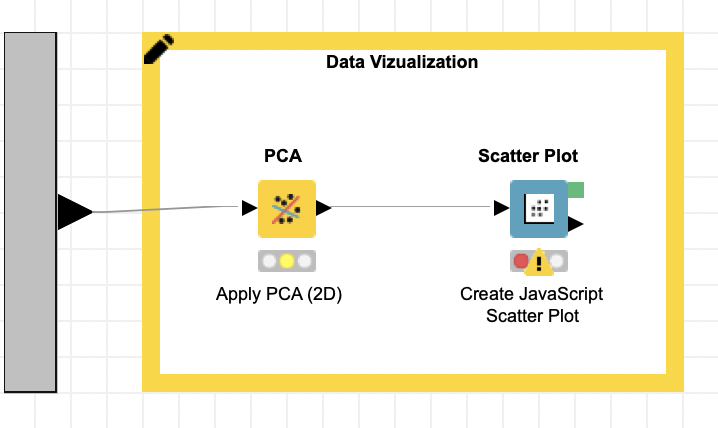
\includegraphics[scale=0.5]{Images/T3.png}
    \caption{Metanodo Data Visualization}
\end{figure}

\subsubsection{Uma Análise de Componentes Principais (PCA) de forma a projetar os dados em
apenas duas dimensões;}

\begin{figure}[H]
    \centering
    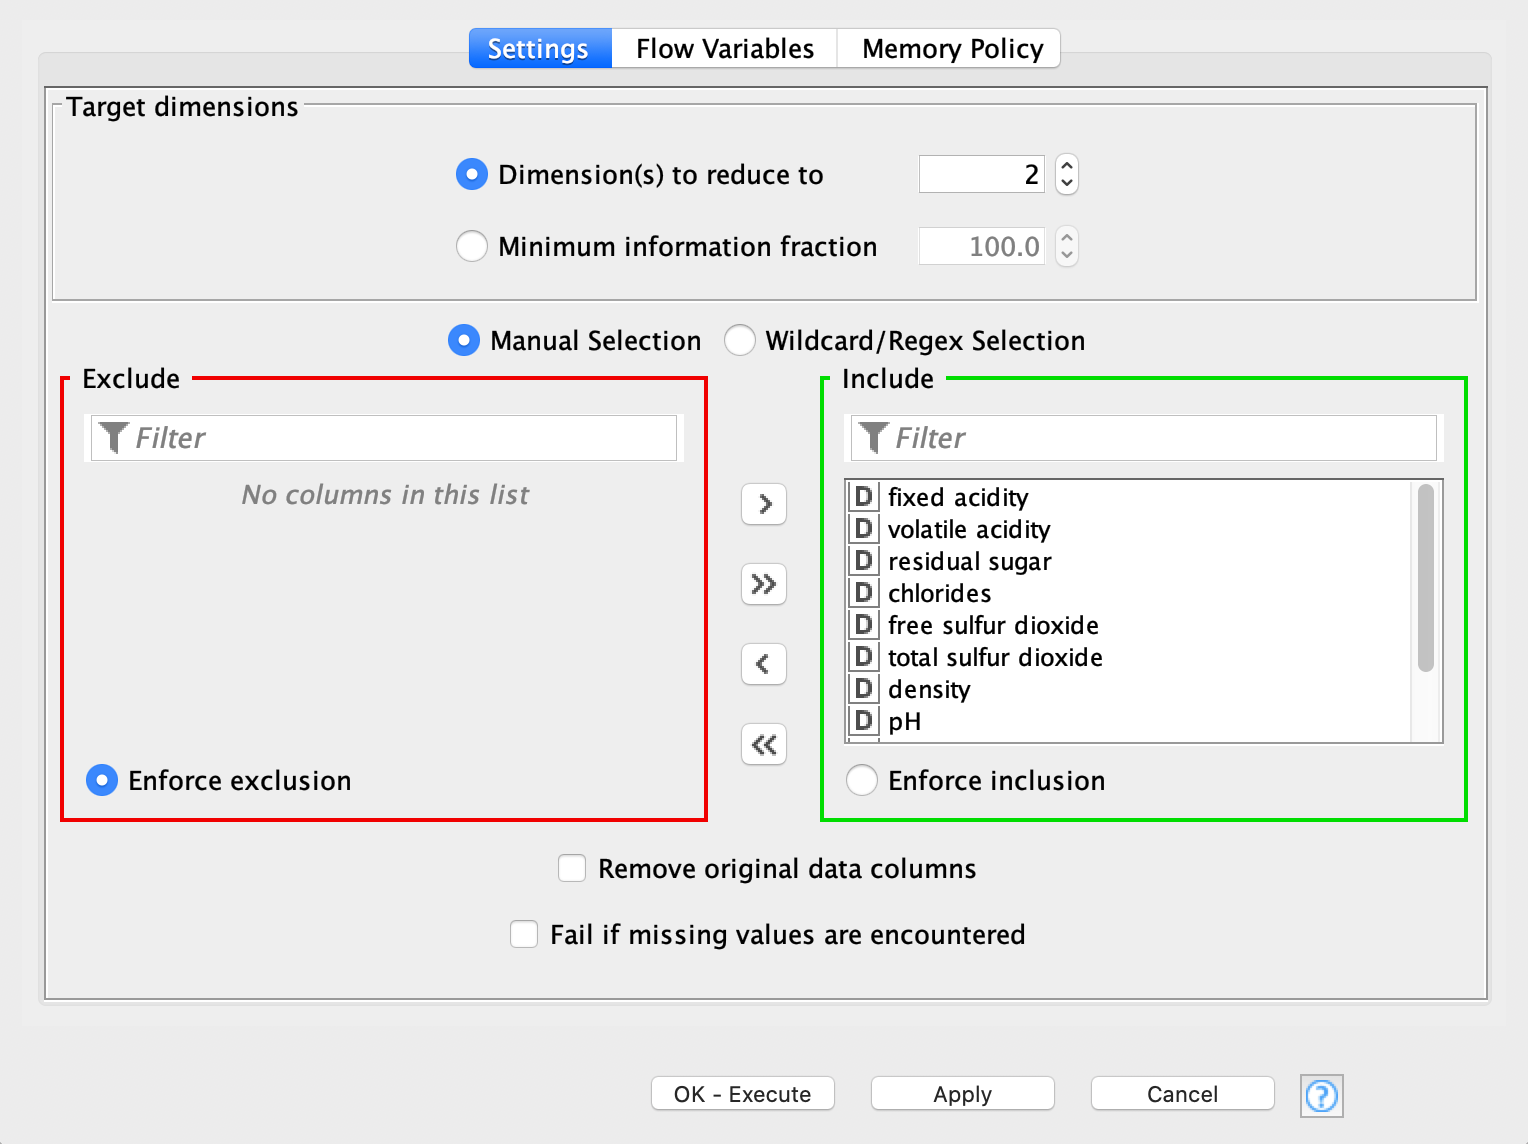
\includegraphics[scale=0.4]{Images/T3_a.png}
    \caption{Aplicação de uma PCA}
\end{figure}

\subsubsection{Utilizar um scatter plot para visualização dos resultados obtidos pelo PCA.}

\begin{figure}[H]
    \centering
    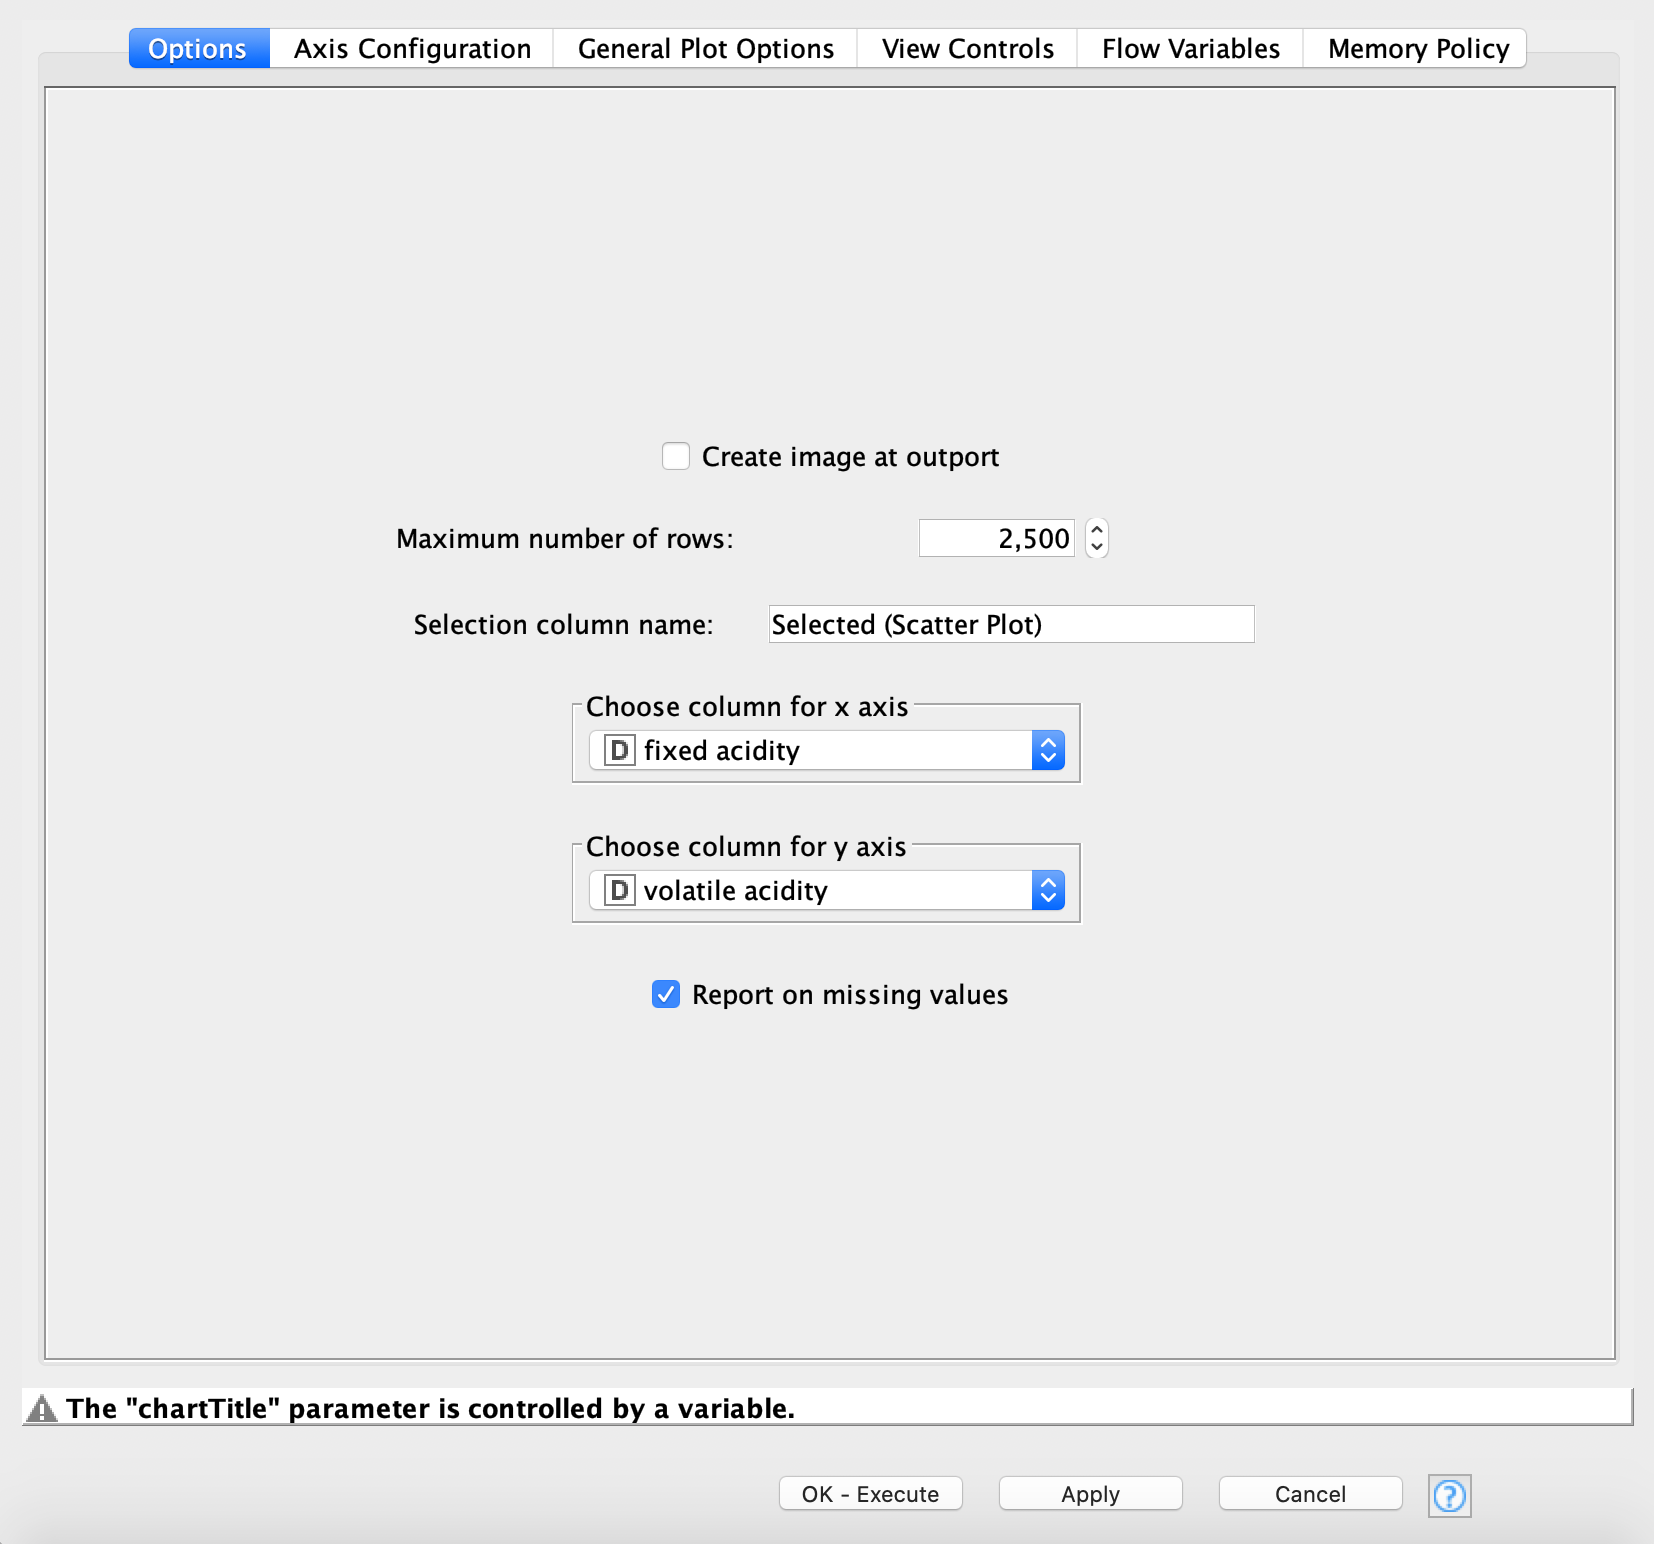
\includegraphics[scale=0.2]{Images/T3_b1.png}
    \caption{Criação do scatter plot}
\end{figure}

\begin{figure}[H]
    \centering
    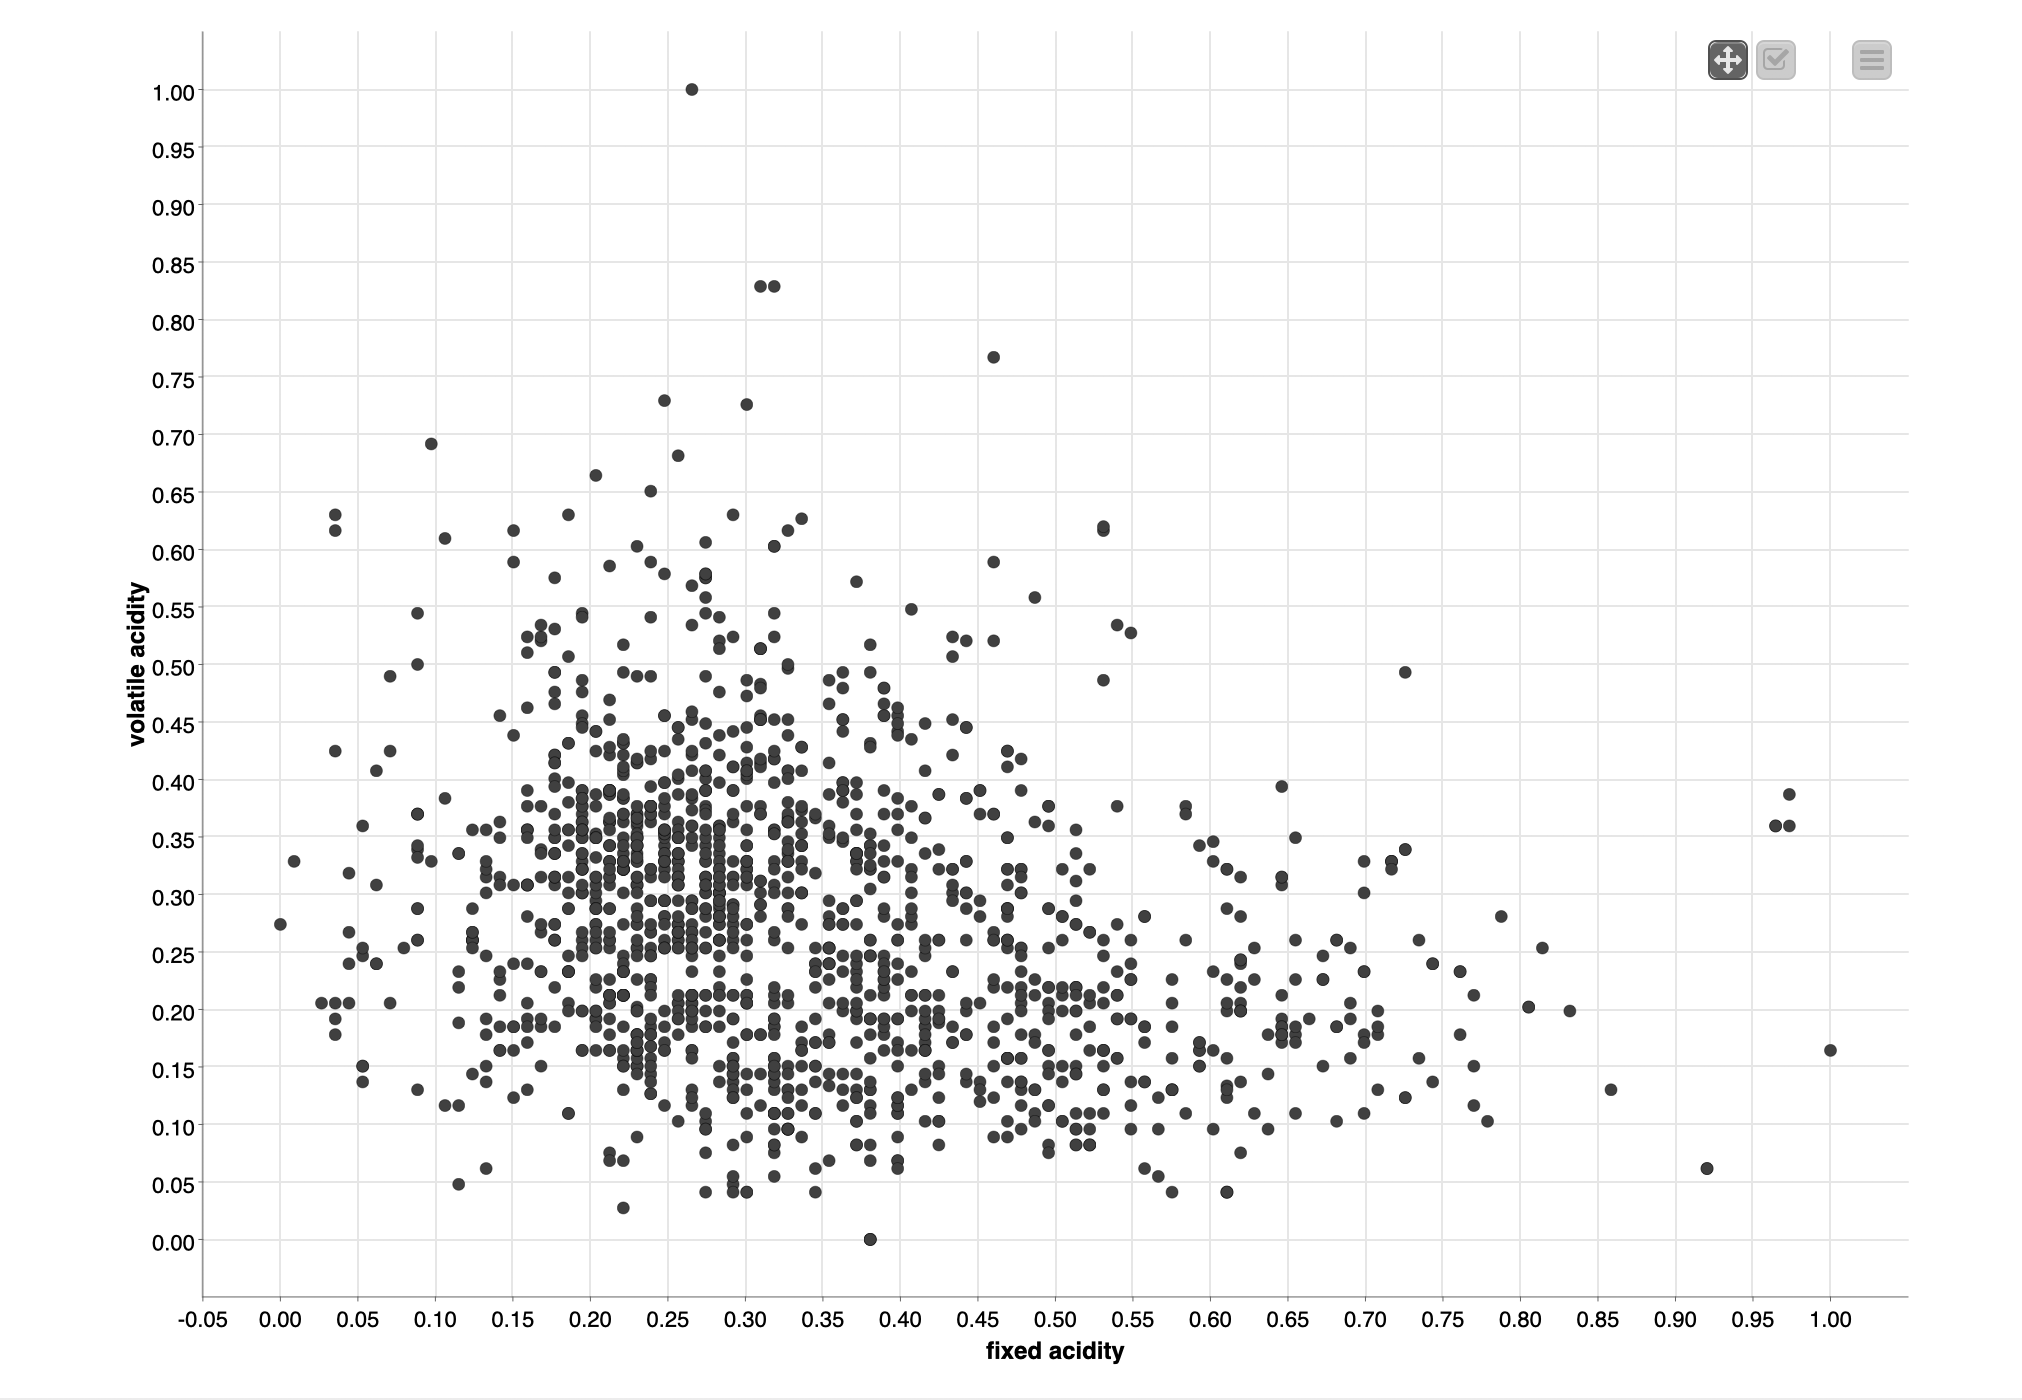
\includegraphics[scale=0.3]{Images/T3_b2.png}
    \caption{Scatter Plot da PCA}
\end{figure}

\clearpage

\section{Tarefa 4}

\subsection{Segmentar o dataset:}

\begin{figure}[H]
    \centering
    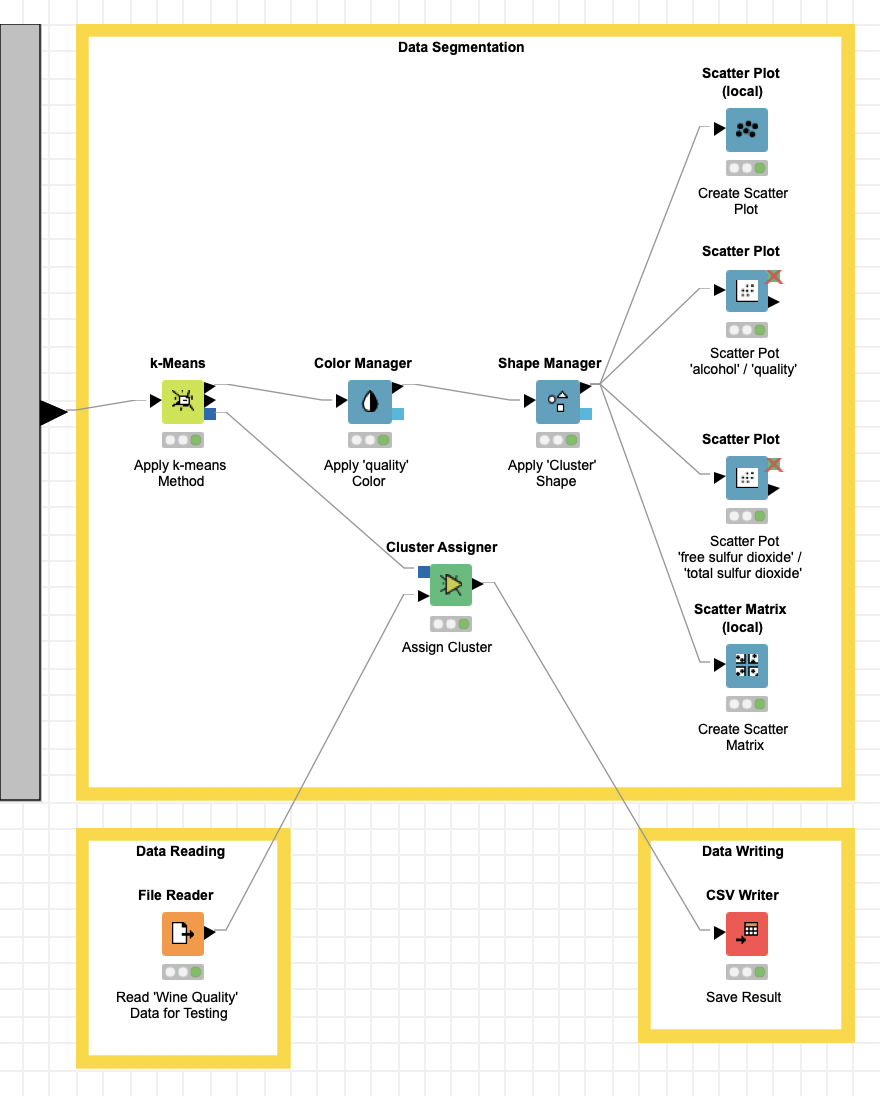
\includegraphics[scale=0.6]{Images/T4.png}
    \caption{Metanode Data Segmentation}
\end{figure}

\subsubsection{Aplicando o método k-means;}

\begin{figure}[H]
    \centering
    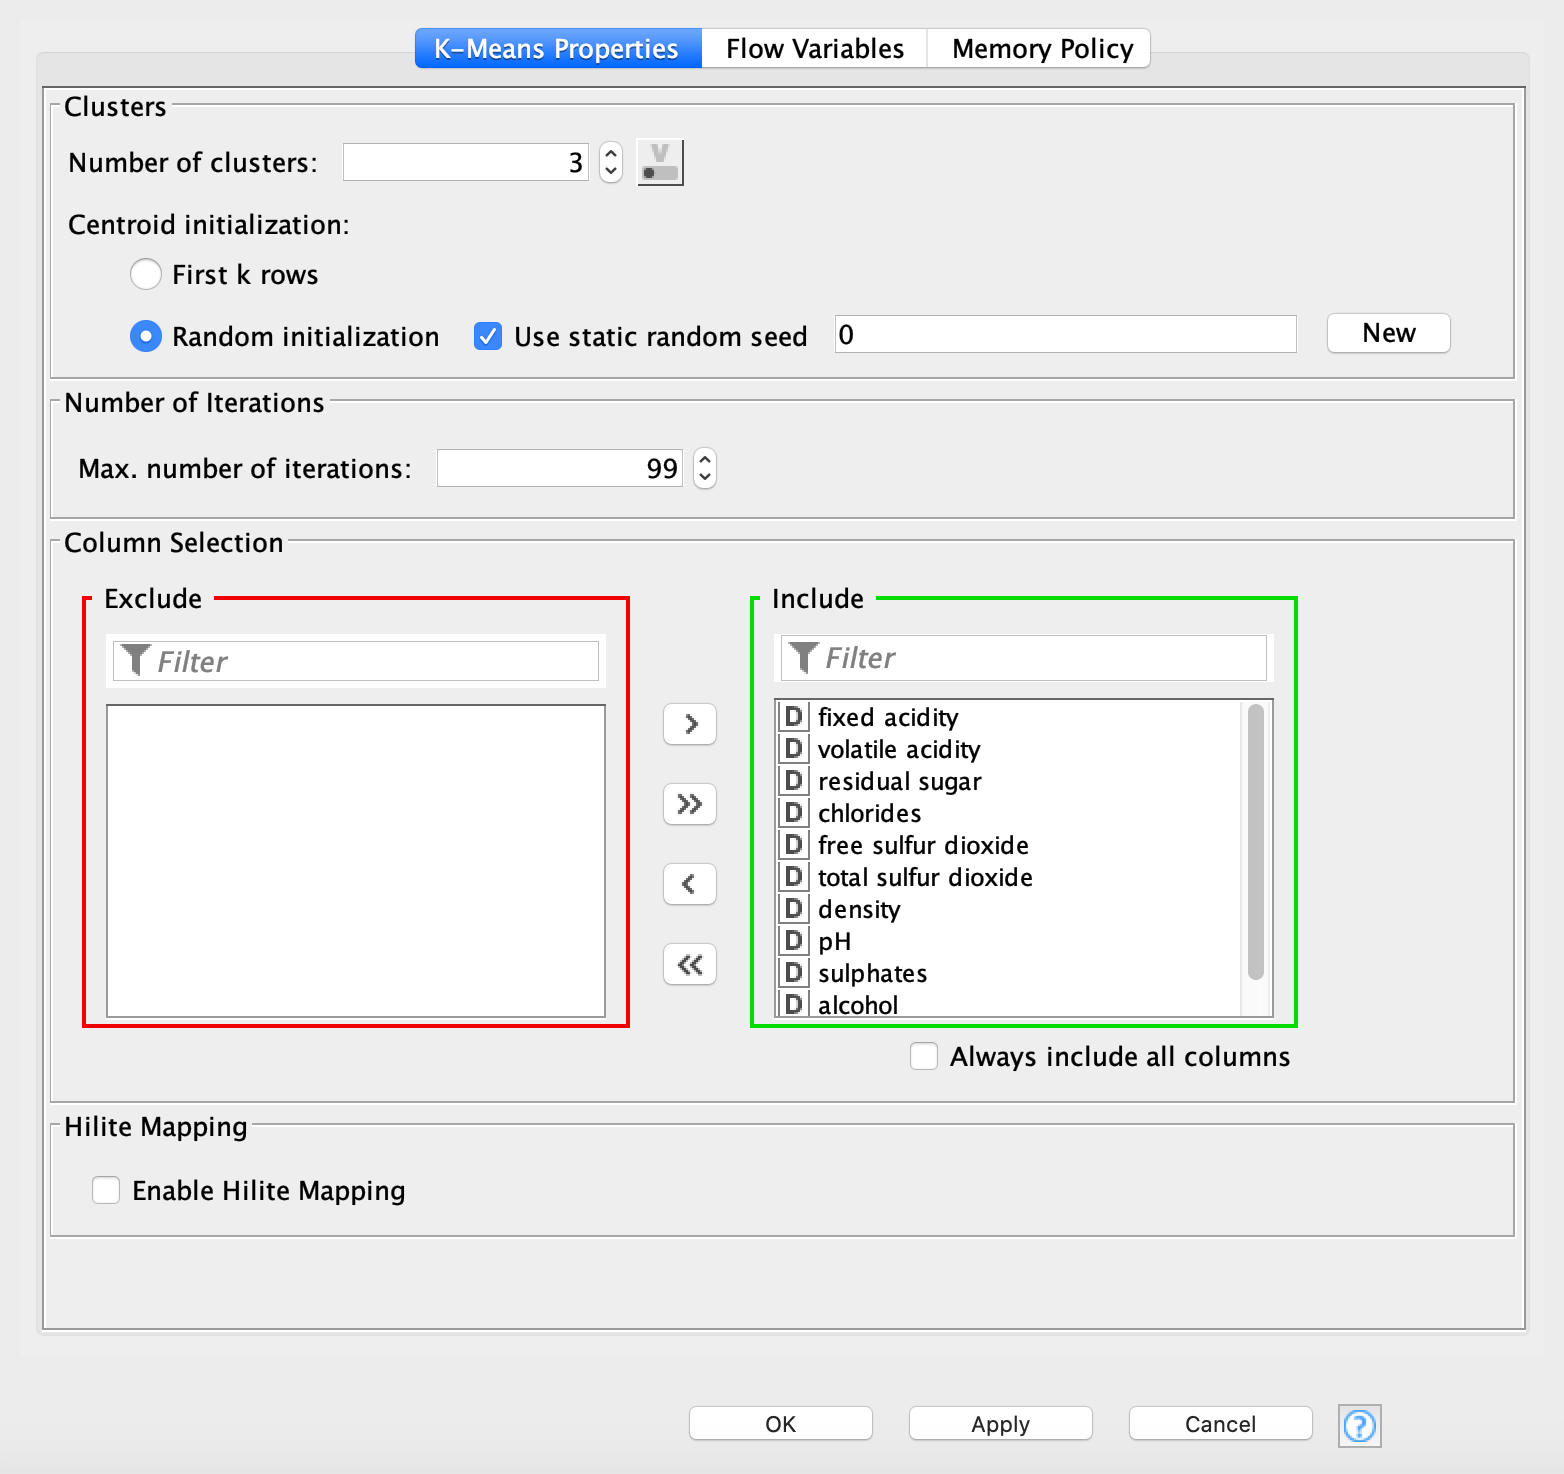
\includegraphics[scale=0.3]{Images/T4_a.png}
    \caption{Método k-means}
\end{figure}

\subsubsection{Atribuir diferentes cores por qualidade do vinho e diferentes formas aos clusters;}

\begin{figure}[H]
    \centering
    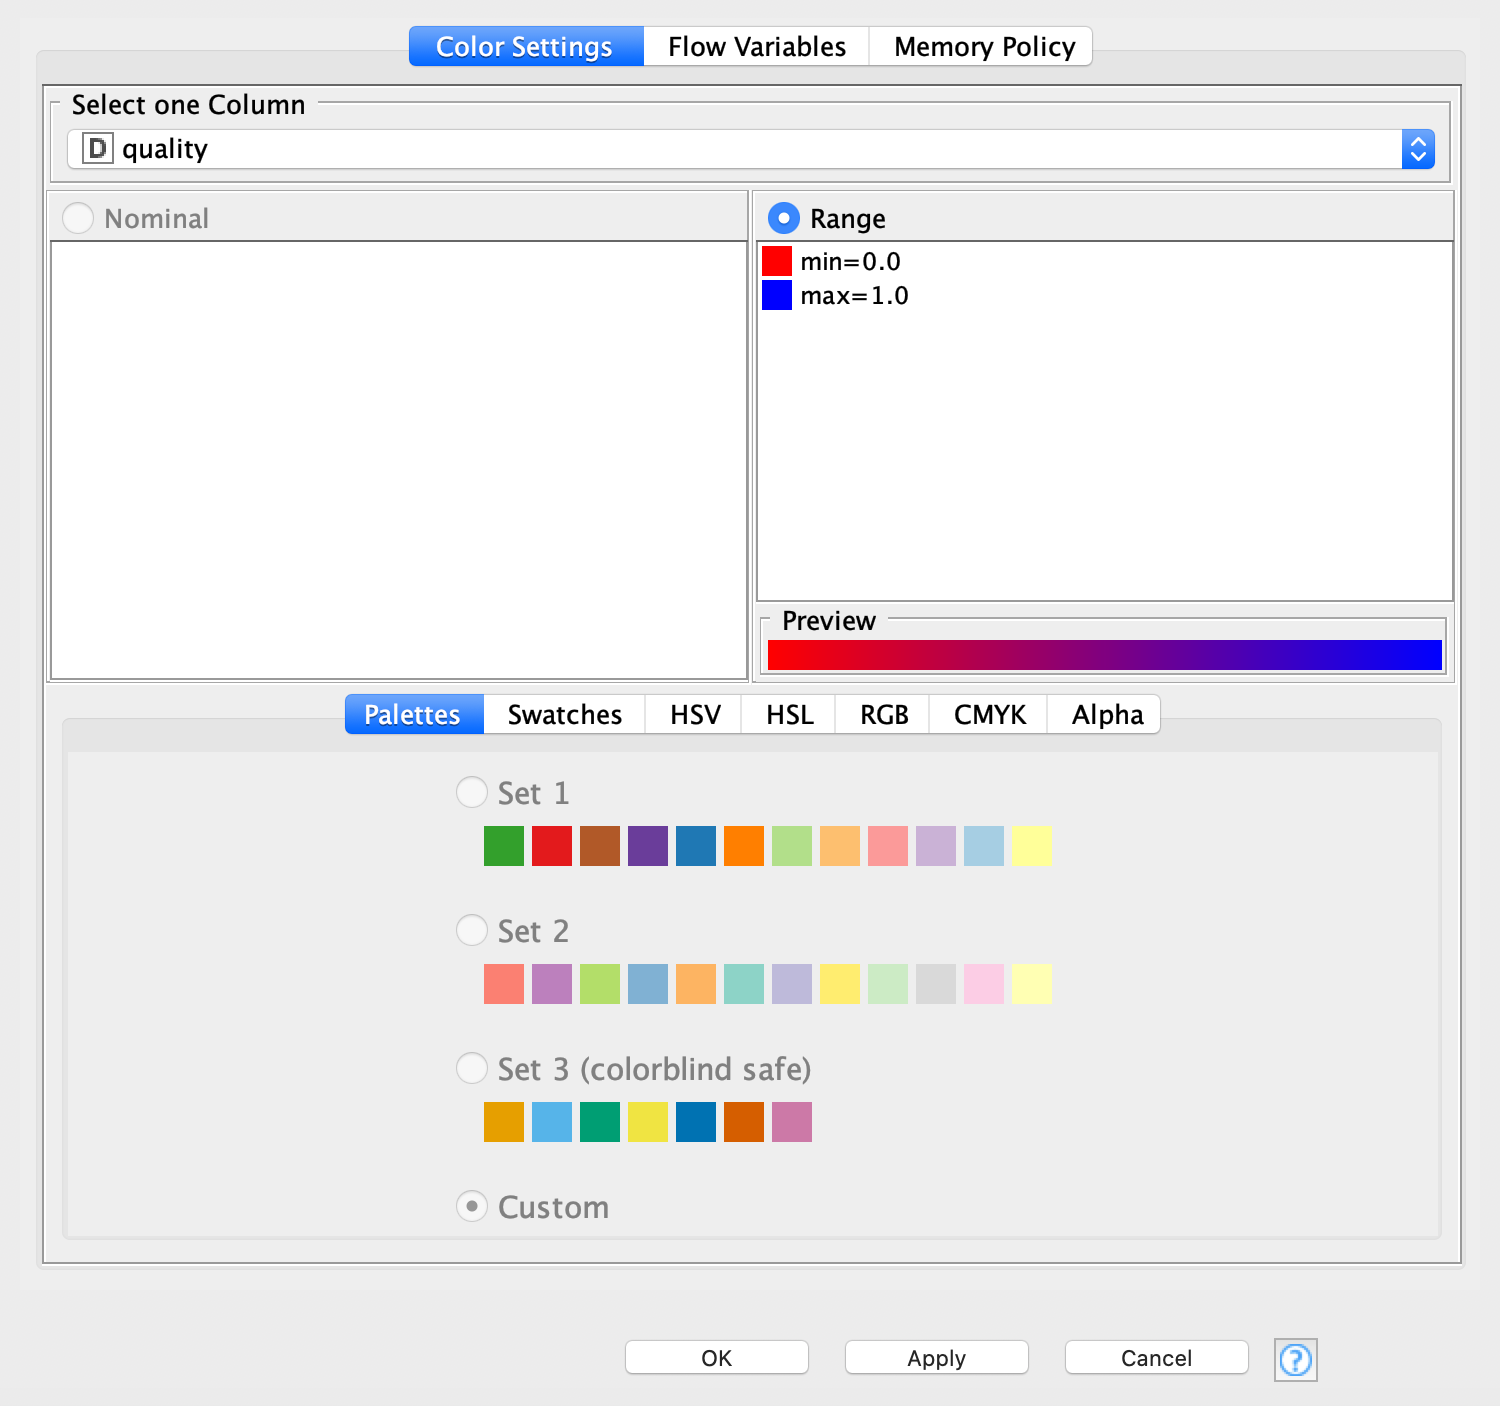
\includegraphics[scale=0.2]{Images/T4_b1.png}
    \caption{Atribuição de cores por qualidade do vinho}
\end{figure}

\begin{figure}[H]
    \centering
    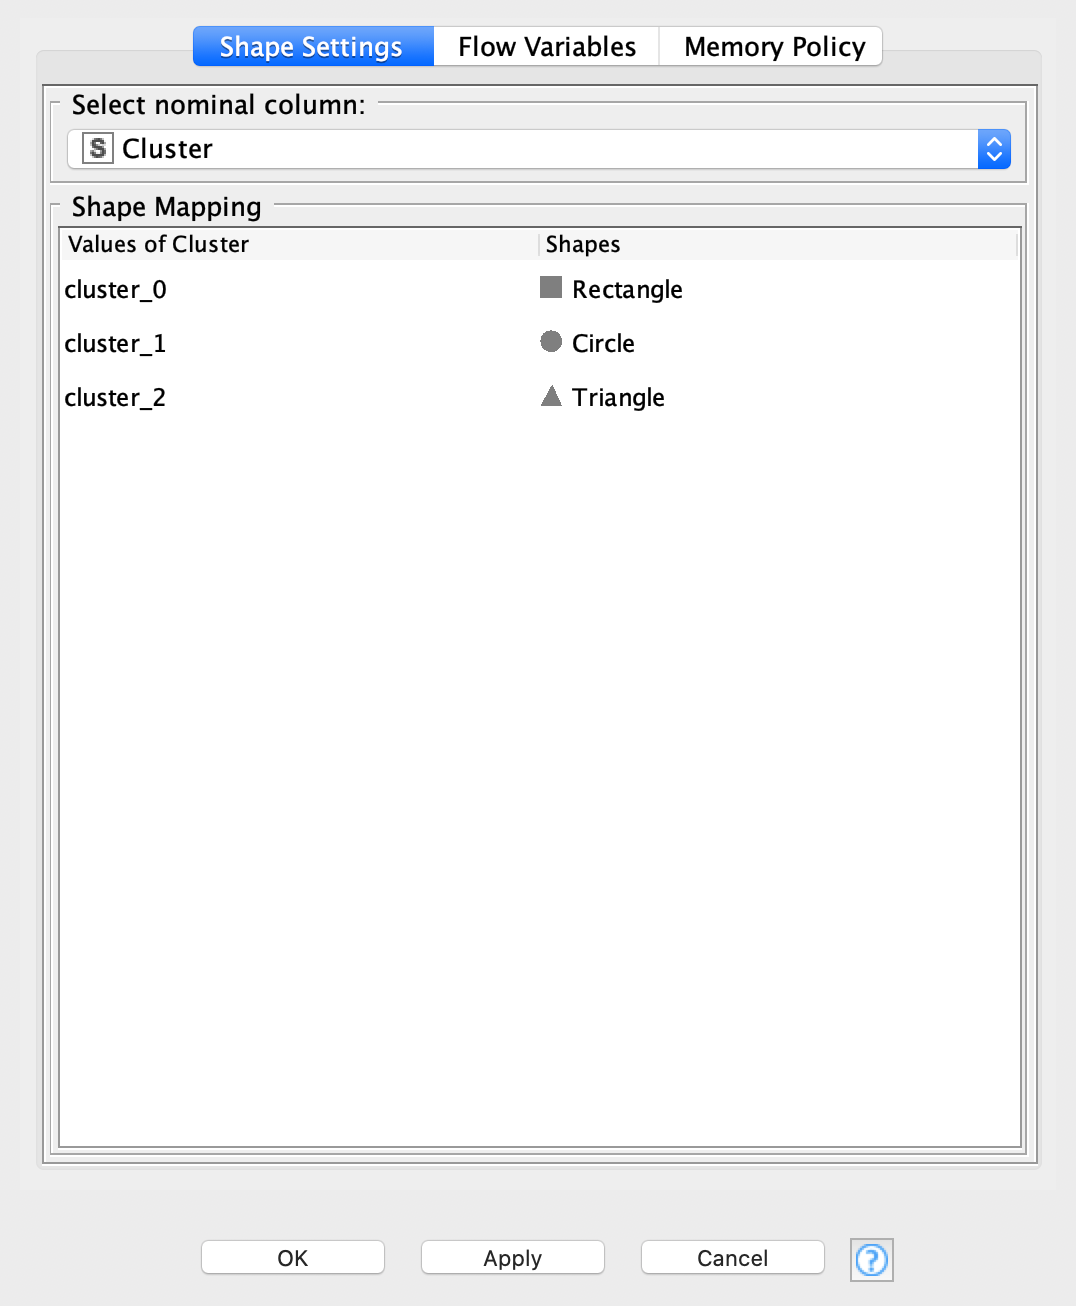
\includegraphics[scale=0.3]{Images/T4_b2.png}
    \caption{Atribuição de formas aos clusters}
\end{figure}

\subsubsection{Criar scatter plots e scatter matrixes que permitam ter uma noção gráfica, em duas dimensões, dos atributos e dos clusters criados;}

\begin{figure}[H]
    \centering
    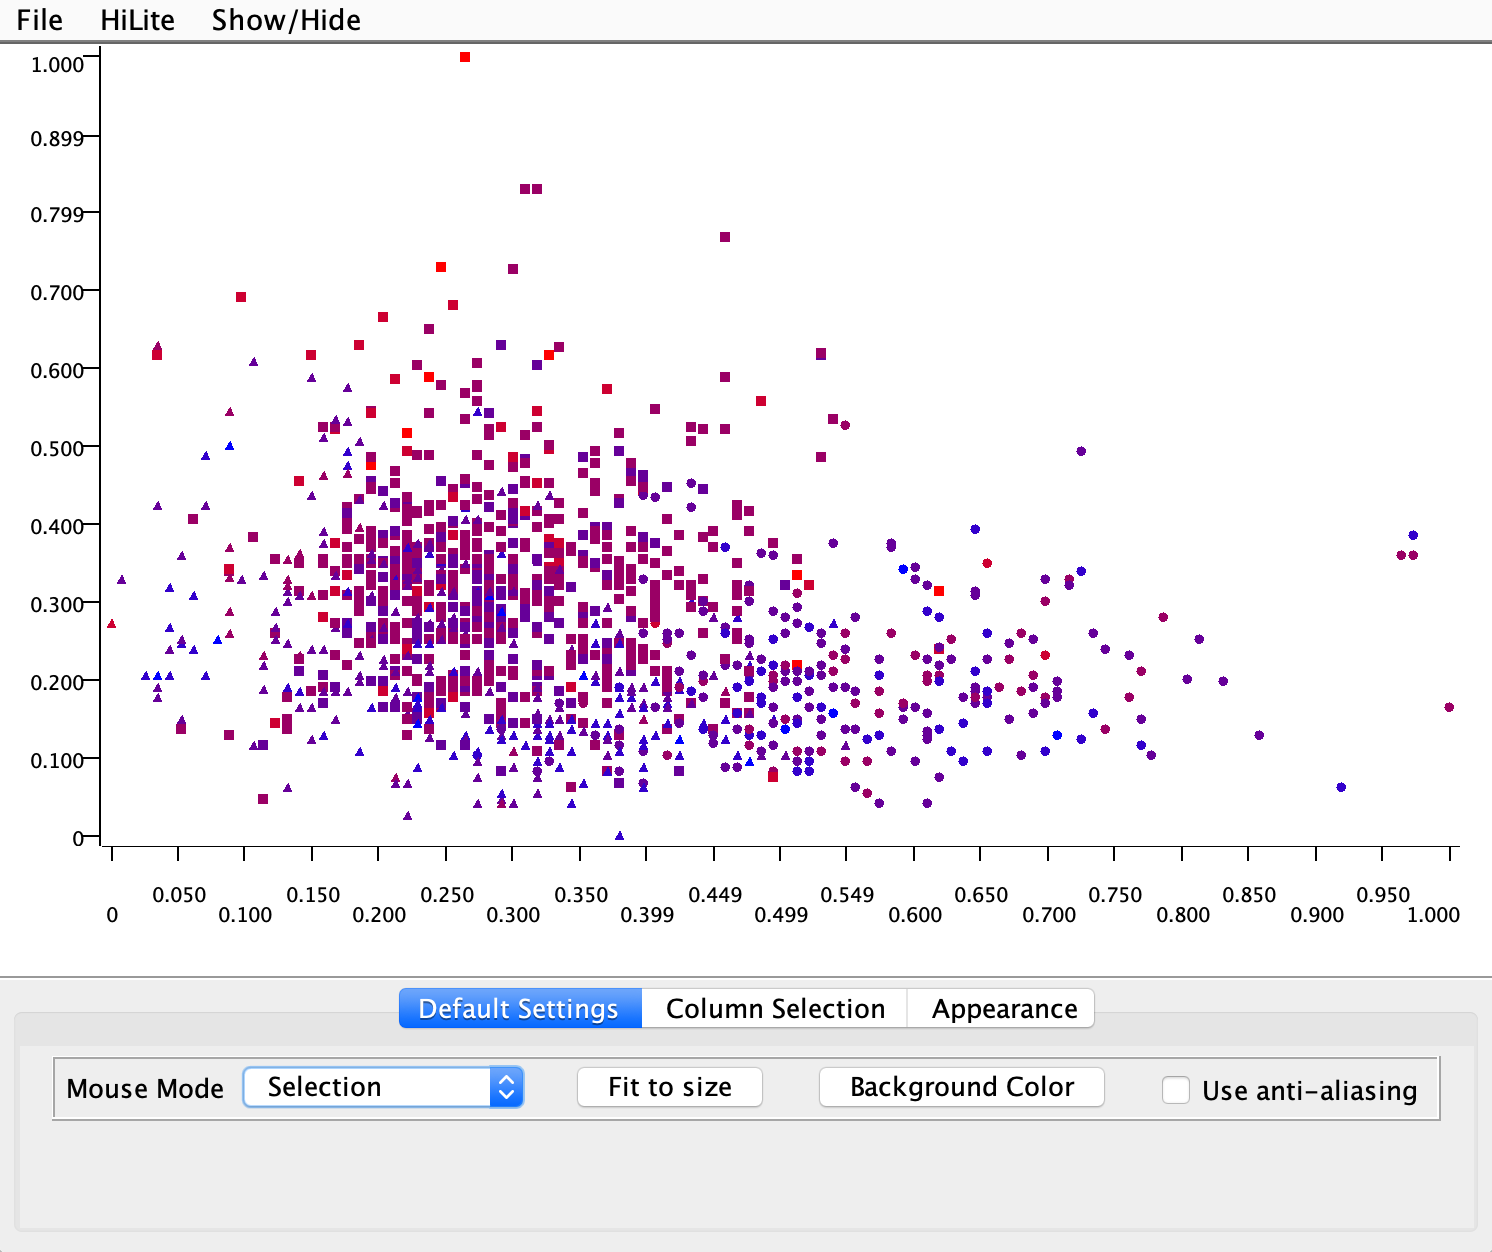
\includegraphics[scale=0.3]{Images/T4_c1.png}
    \caption{Scatter plot}
\end{figure}

\begin{figure}[H]
    \centering
    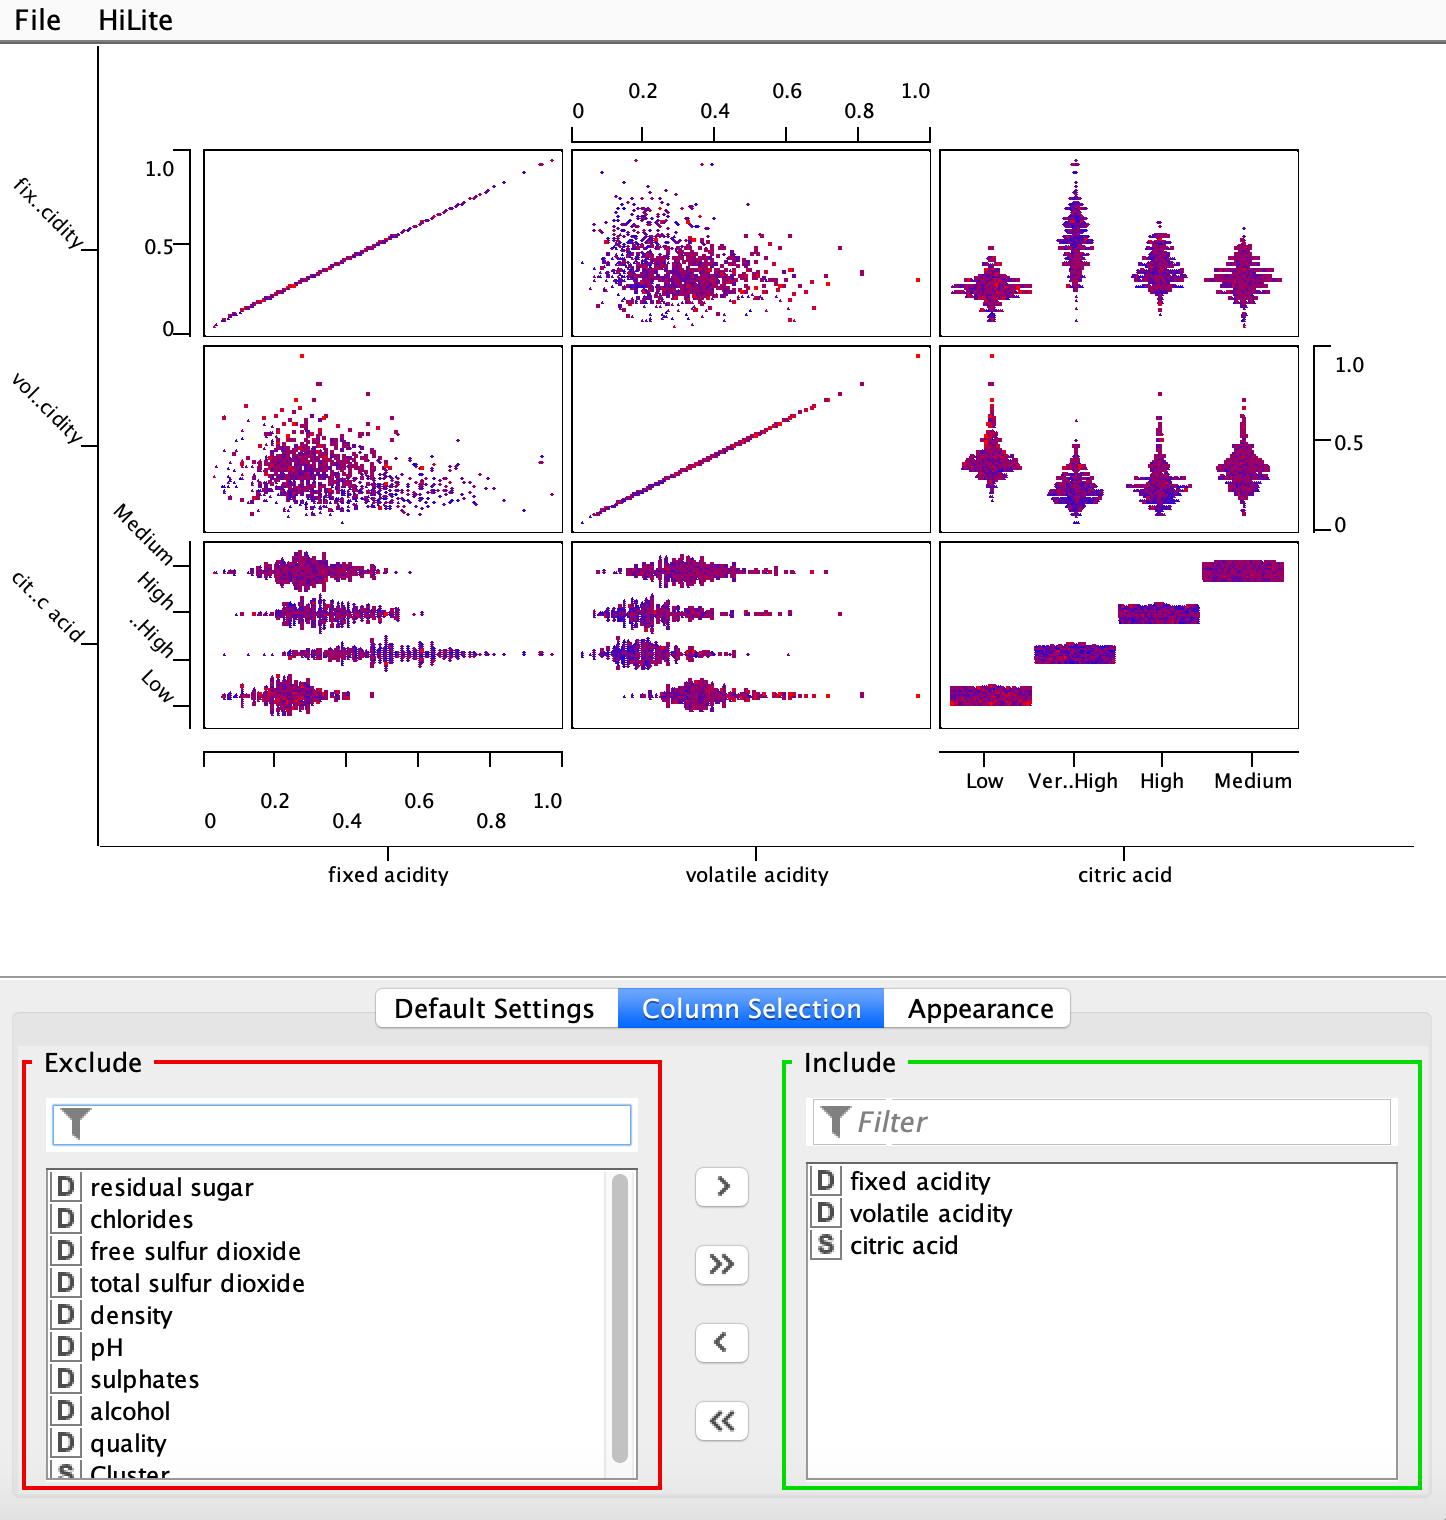
\includegraphics[scale=0.4]{Images/T4_c2.png}
    \caption{Scatter Matrix}
\end{figure}

\subsubsection{Ler e tratar os dados de teste de forma a que, com base no modelo desenvolvido nos passos anteriores, seja atribuído um cluster a cada registo deste ficheiro;}

\begin{figure}[H]
    \centering
    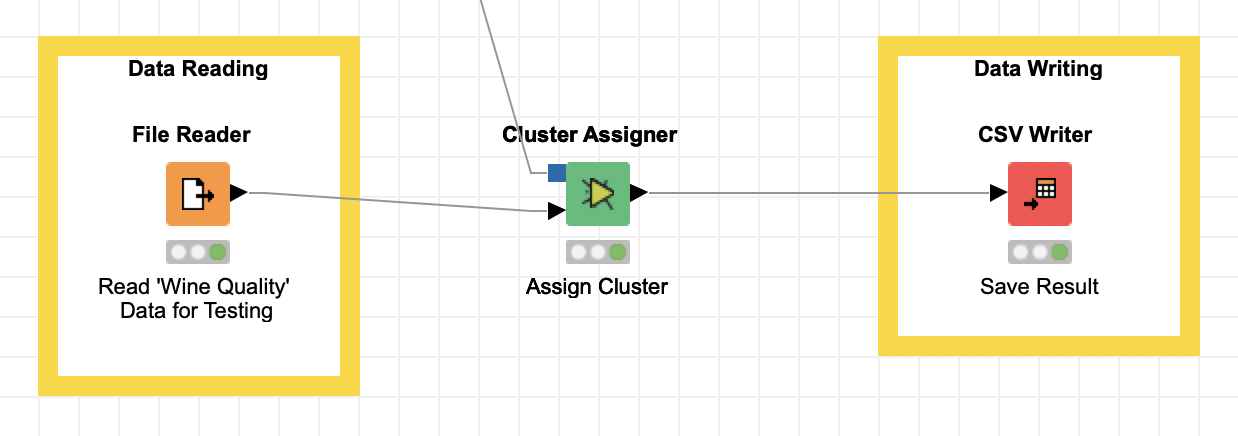
\includegraphics[scale=0.4]{Images/T4_d.png}
    \caption{Leitura dos dados de teste e aplicação do modelo desenvolvido}
\end{figure}

\subsubsection{Guardar o resultado da atribuição num ficheiro csv.}

\begin{figure}[H]
    \centering
    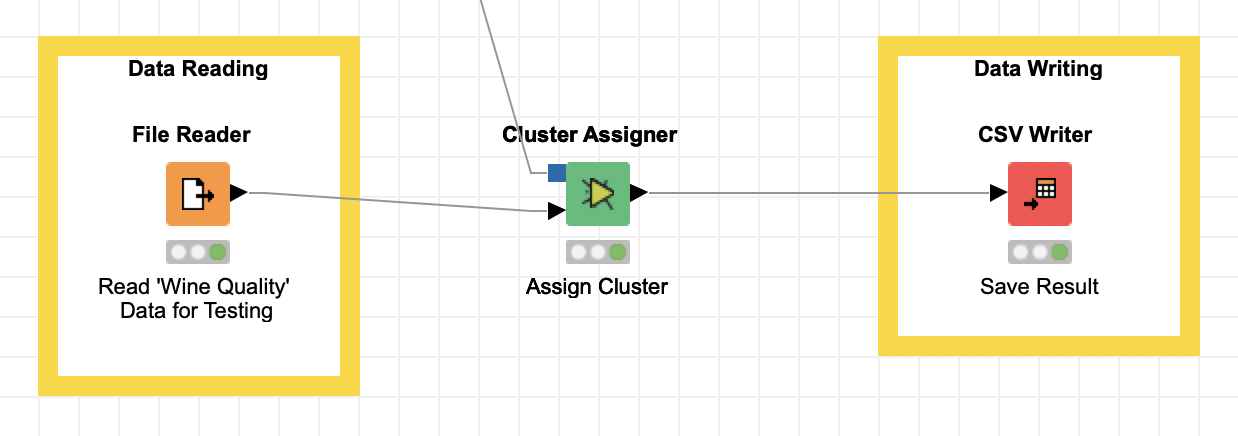
\includegraphics[scale=0.4]{Images/T4_d.png}
    \caption{Guardar o resultado}
\end{figure}

\clearpage

\section{Tarefa 5}

\subsection{Parametrizar o workflow, utilizando variáveis de fluxo para definir o número de bins, o número de clusters e os títulos dos gráficos criados;}

\begin{figure}[H]
    \centering
    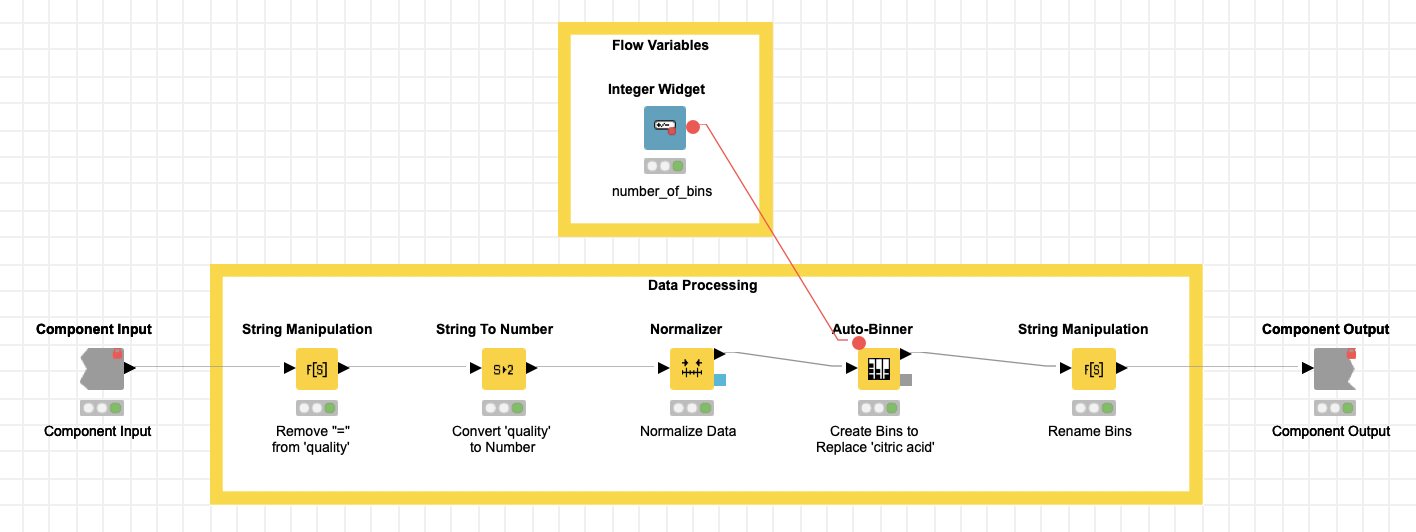
\includegraphics[scale=0.4]{Images/T5_a.png}
    \caption{Variável para o número de bins}
\end{figure}

\begin{figure}[H]
    \centering
    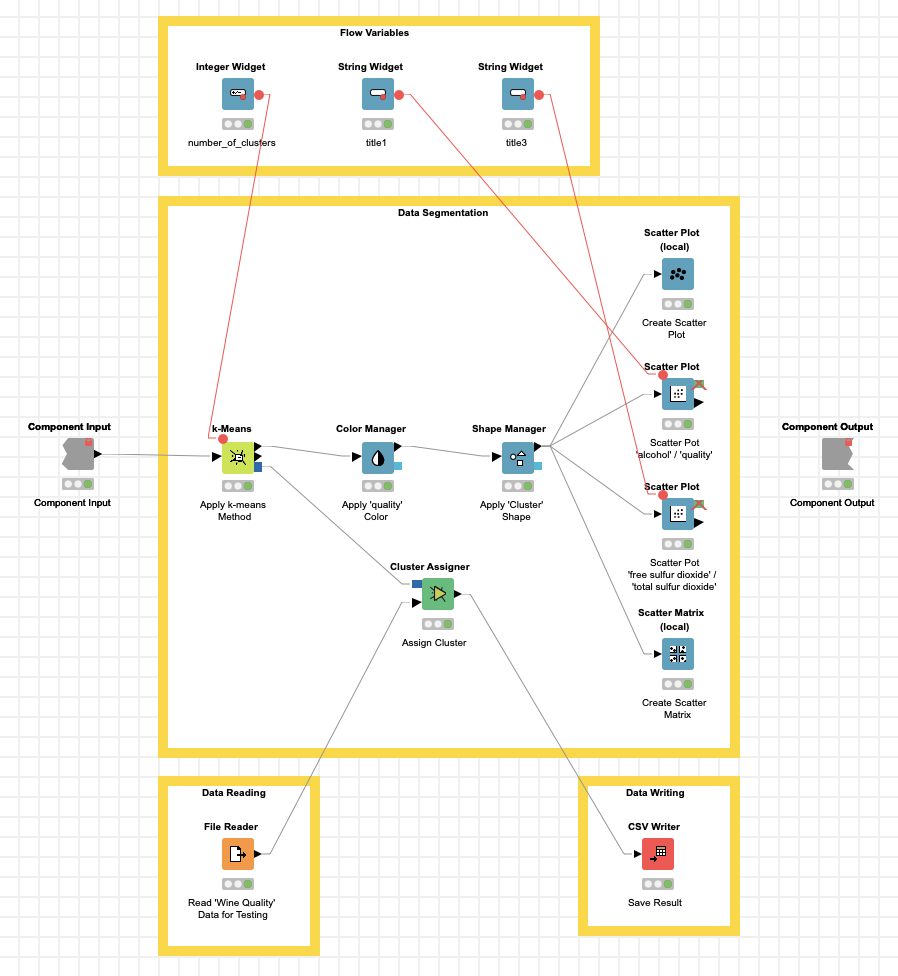
\includegraphics[scale=0.4]{Images/T5_b.png}
    \caption{Variáveis para o número de clusters e os títulos dos gráficos}
\end{figure}

\clearpage

\section{Tarefa 6}

\subsection{Produzir o workflow de maneira a que seja possível visualizar, numa única página, todos os componentes visuais implementados;}

\begin{figure}[H]
    \centering
    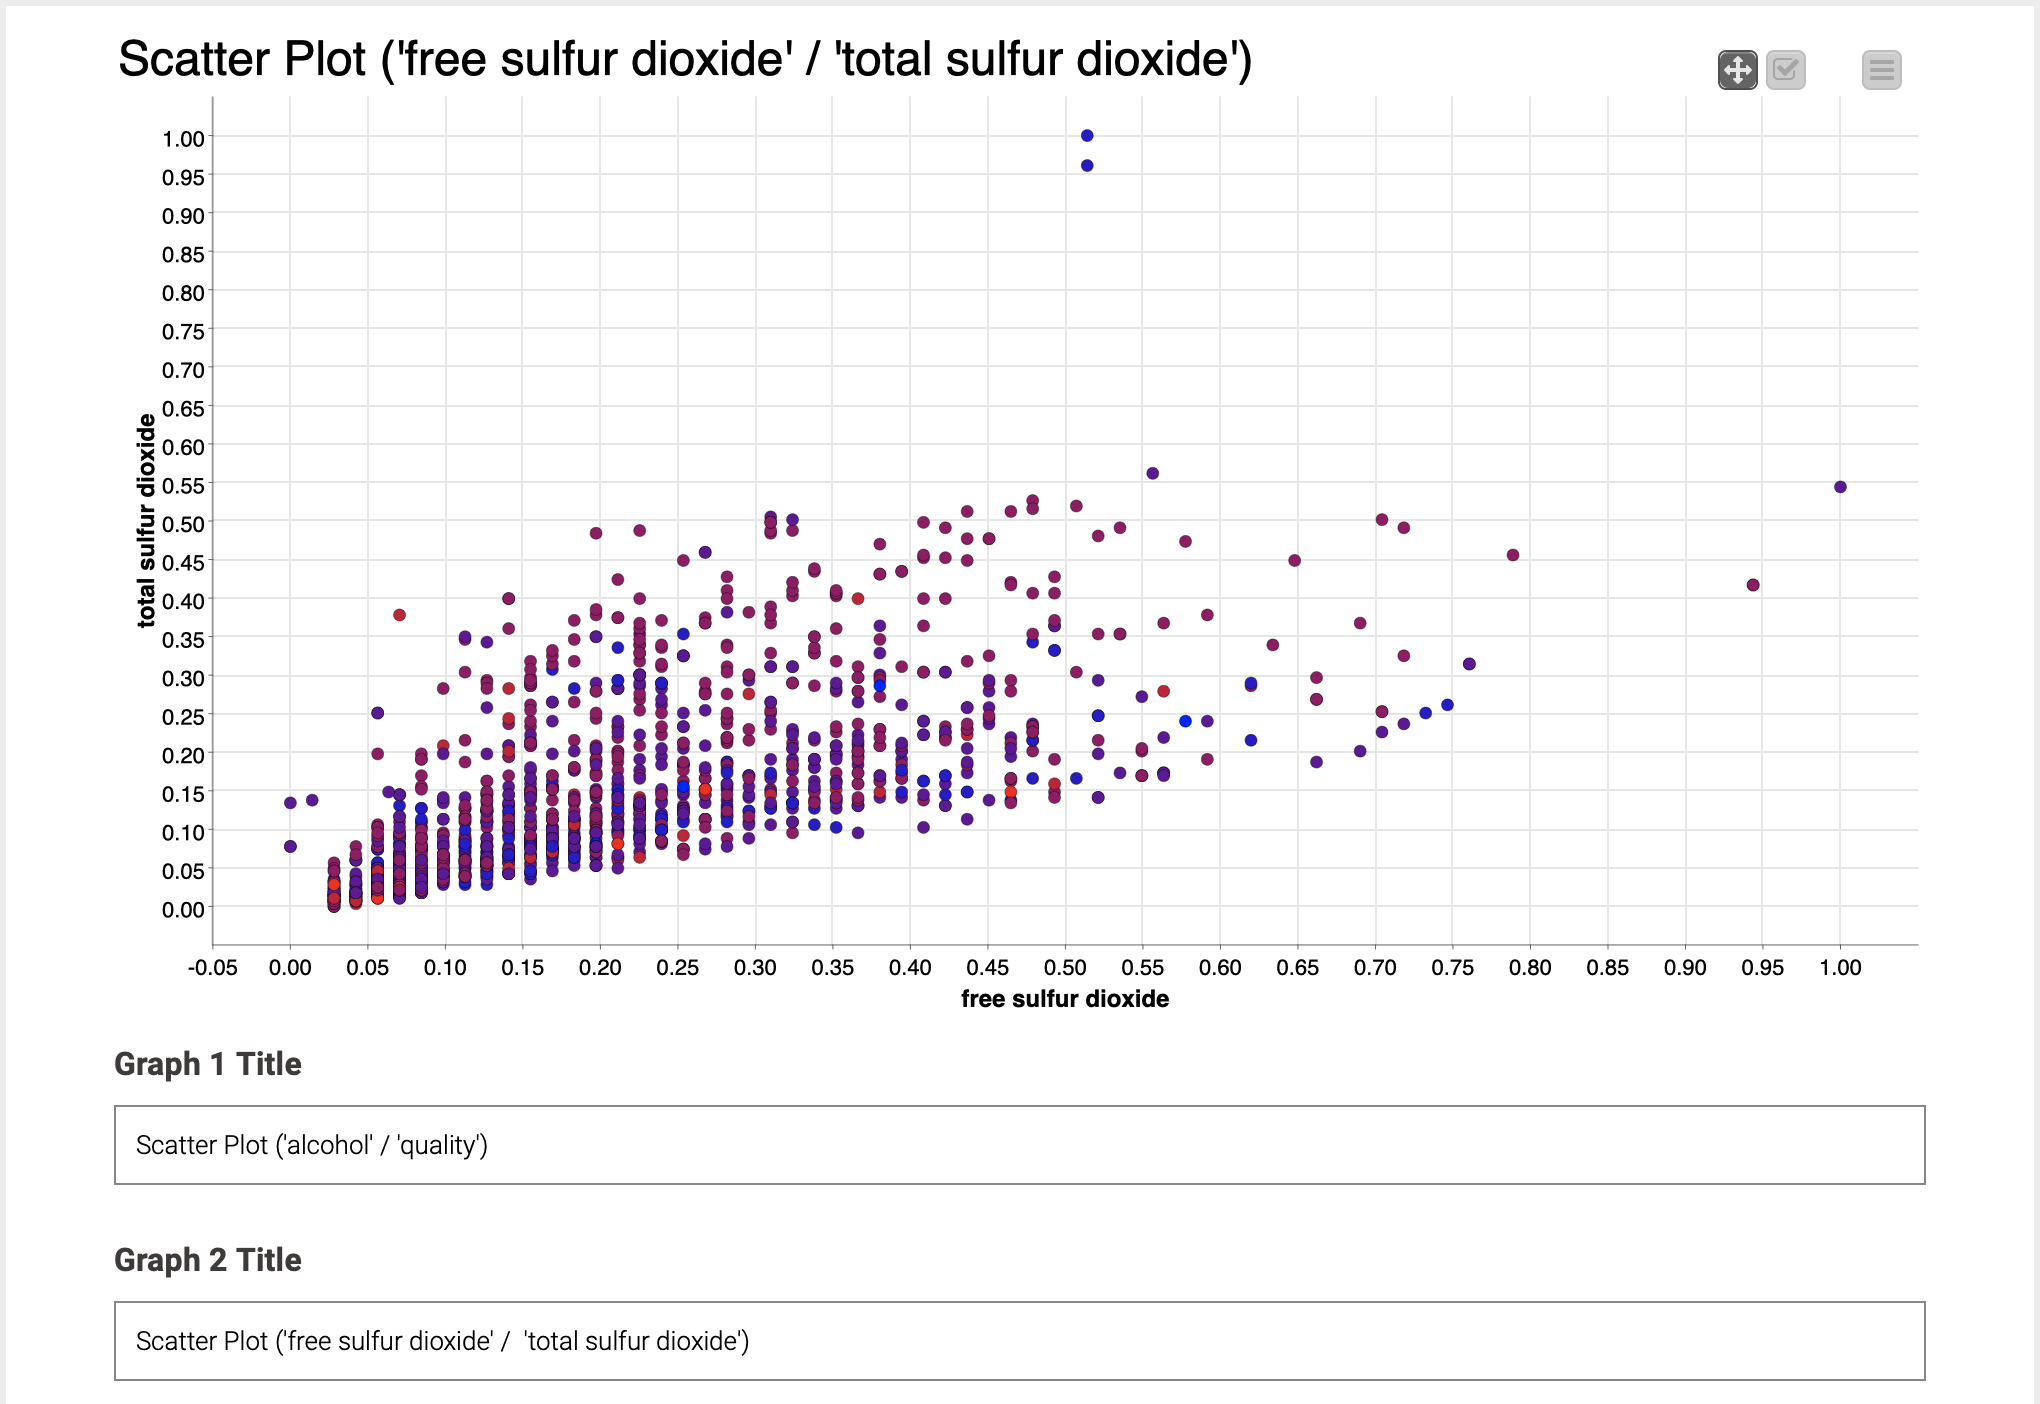
\includegraphics[scale=0.3]{Images/T6_a.png}
    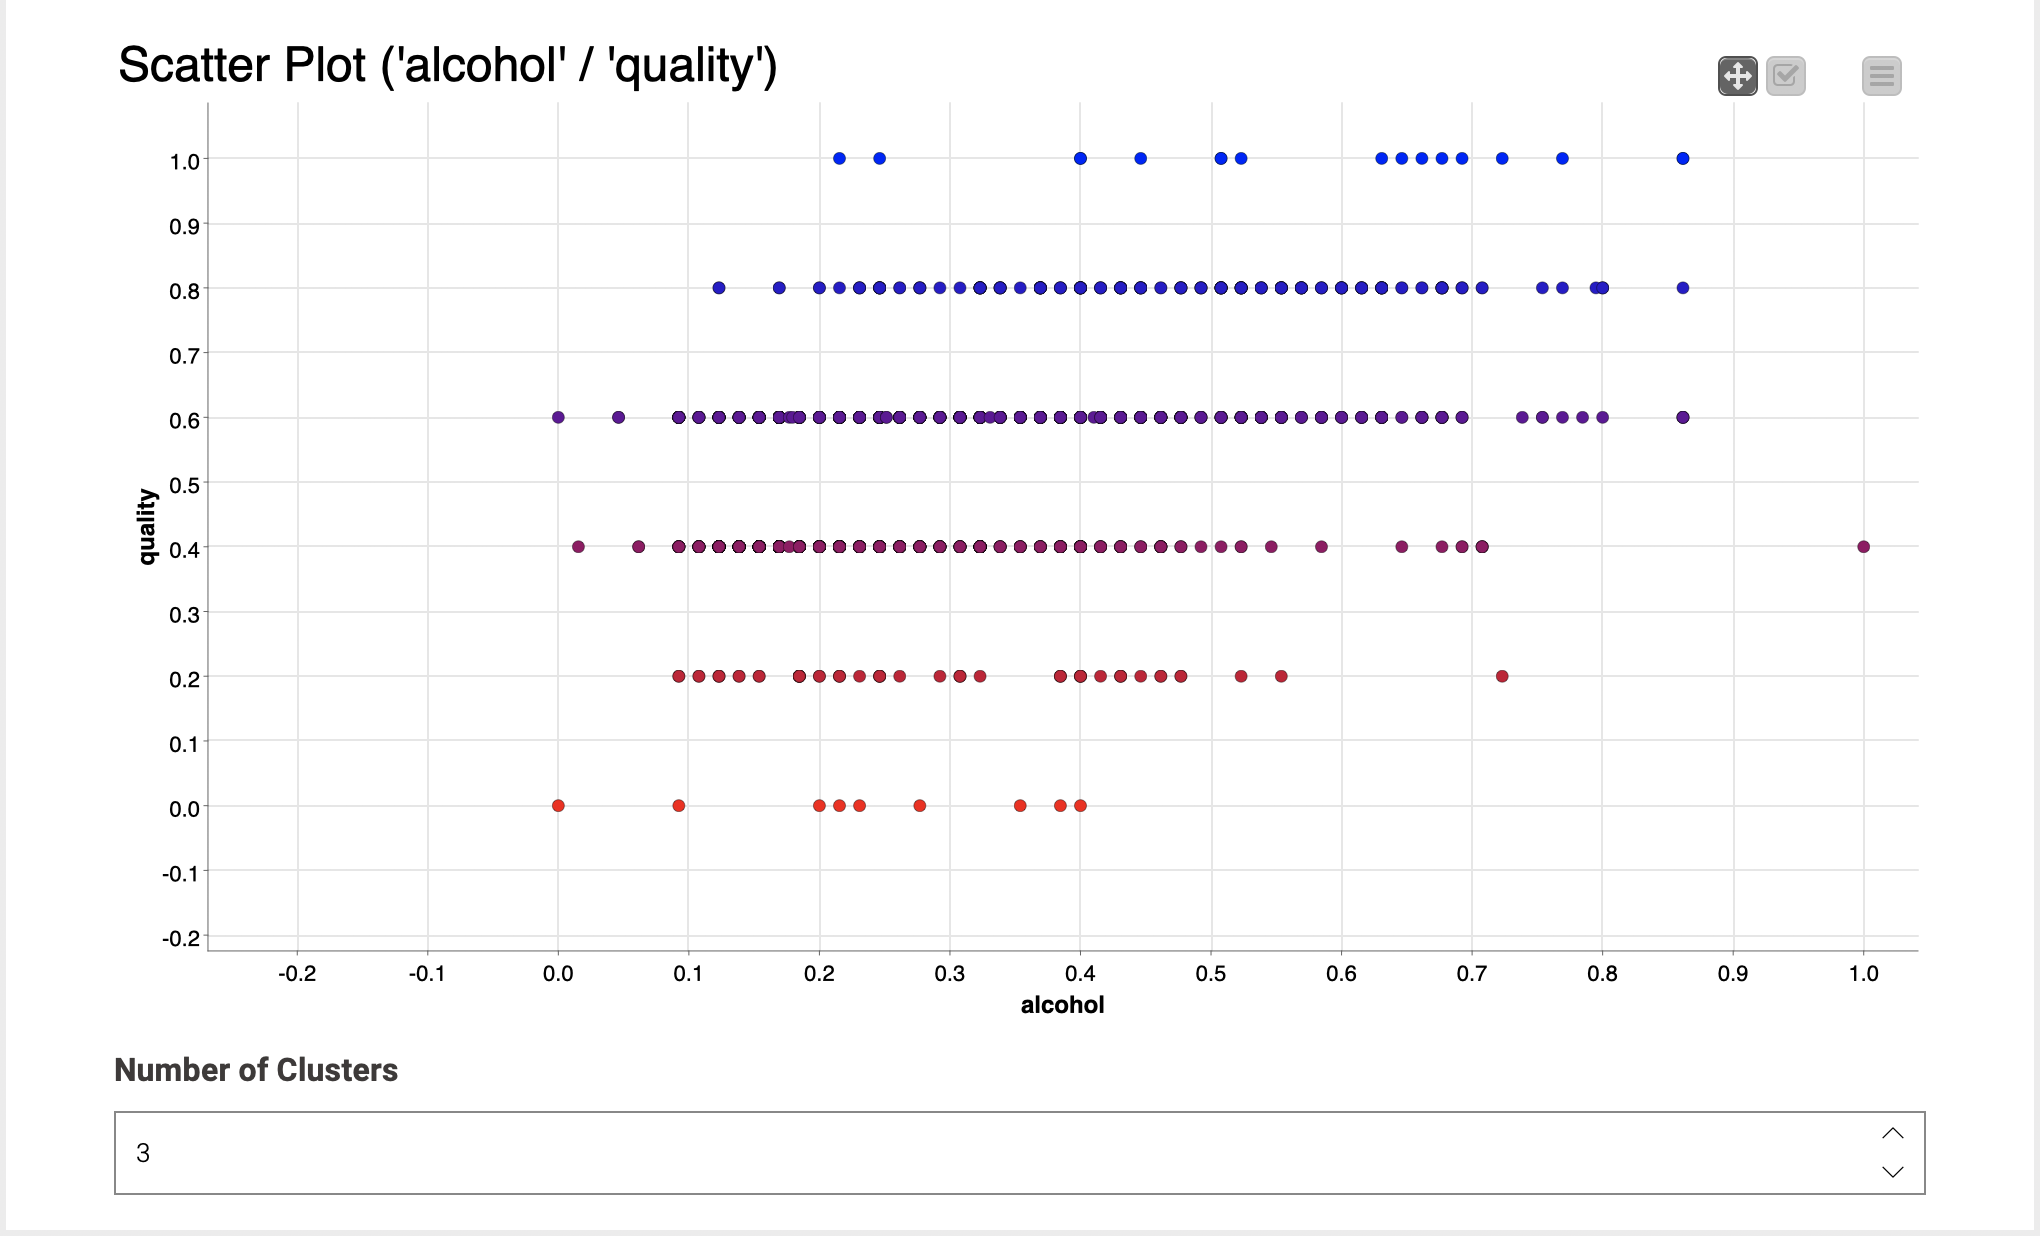
\includegraphics[scale=0.3]{Images/T6_b.png}
    \caption{Página com os componentes visuais}
\end{figure}

\clearpage

\section{Tarefa 7}

\subsection{Experimentar, avaliar e comparar outros métodos de segmentação.}

\begin{figure}[H]
    \centering
    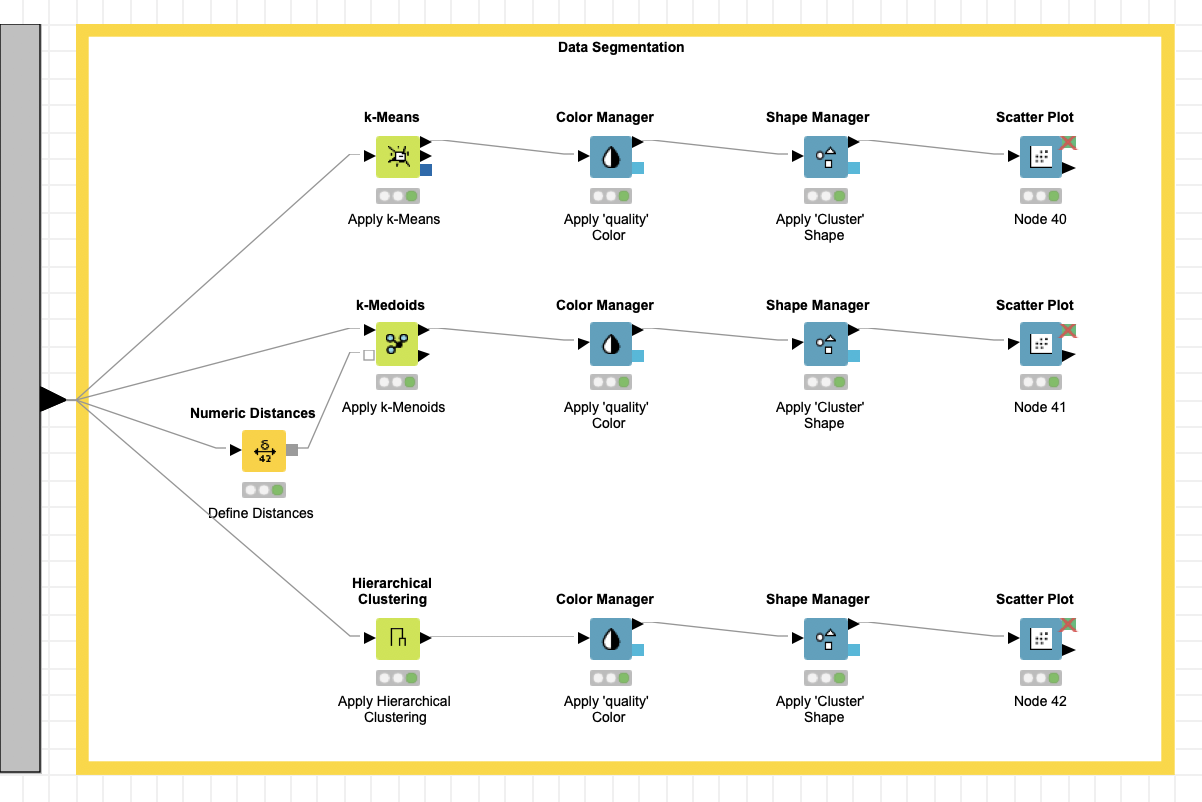
\includegraphics[scale=0.4]{Images/T7.png}
    \caption{Metanodos de Segmentação}
\end{figure}

\subsubsection{Particionamento}

Método k-Means: Apesar de ser relativamente eficiente e terminar com ótimos locais, apenas é aplicável quando é possível calcular a média, necessita da identificação do número de segmentos à priori, é incapaz de lidar com ruído e é inadequado para a determinação de segmentos côncavos. \\
\\
Método k-Menoids: Apesar de apresentar maior robustez relativamente à presença de dados ruidosos comparativamente ao método k-Means, a qualidade dos resultados diminui quanto maior a dimensão dos conjuntos de dados.

\subsubsection{Hierarquização}

Comparativamente ao método k-Means, apresenta melhor resultados e não necessita da especificação do número de segmentos.
Ao contrário do particionamento, traduz alguma organização dos segmentos em vez de um simples conjunto de segmentos.
Contudo, apresenta dificuldades com o aumento de atributos ou objetos.

\begin{figure}[H]
    \centering
    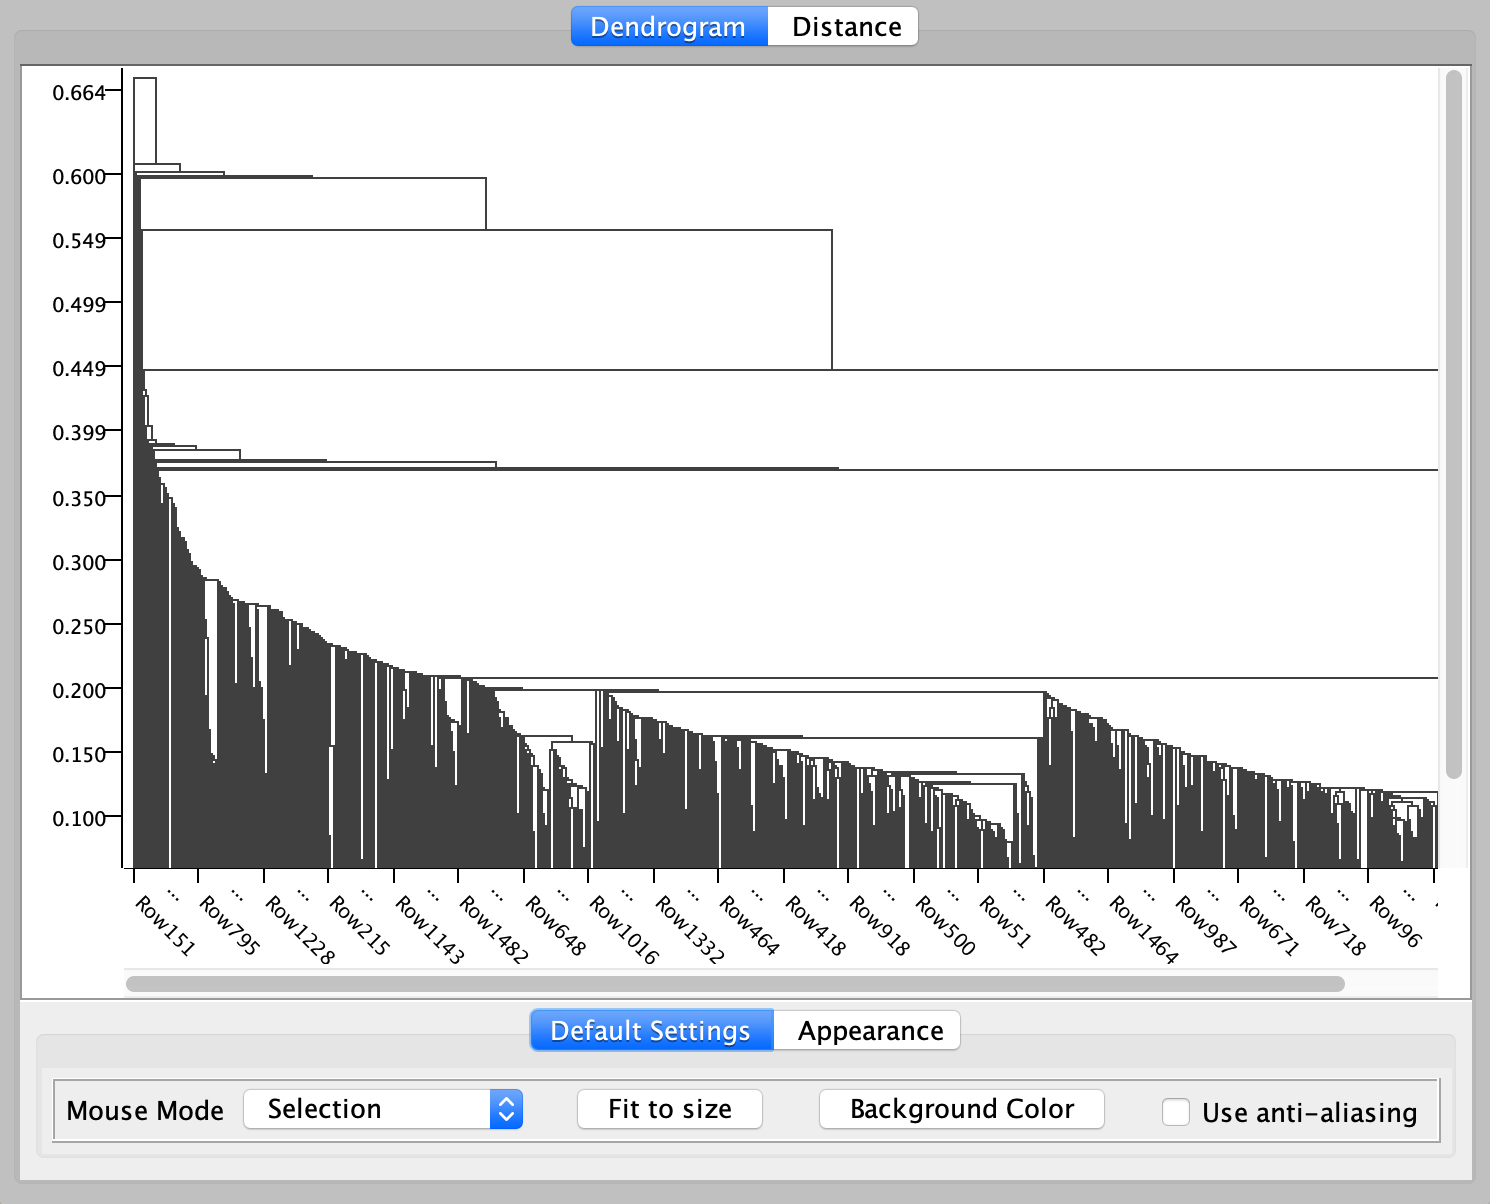
\includegraphics[scale=0.3]{Images/T7_a.png}
    \caption{Dendograma}
\end{figure}

\begin{figure}[H]
    \centering
    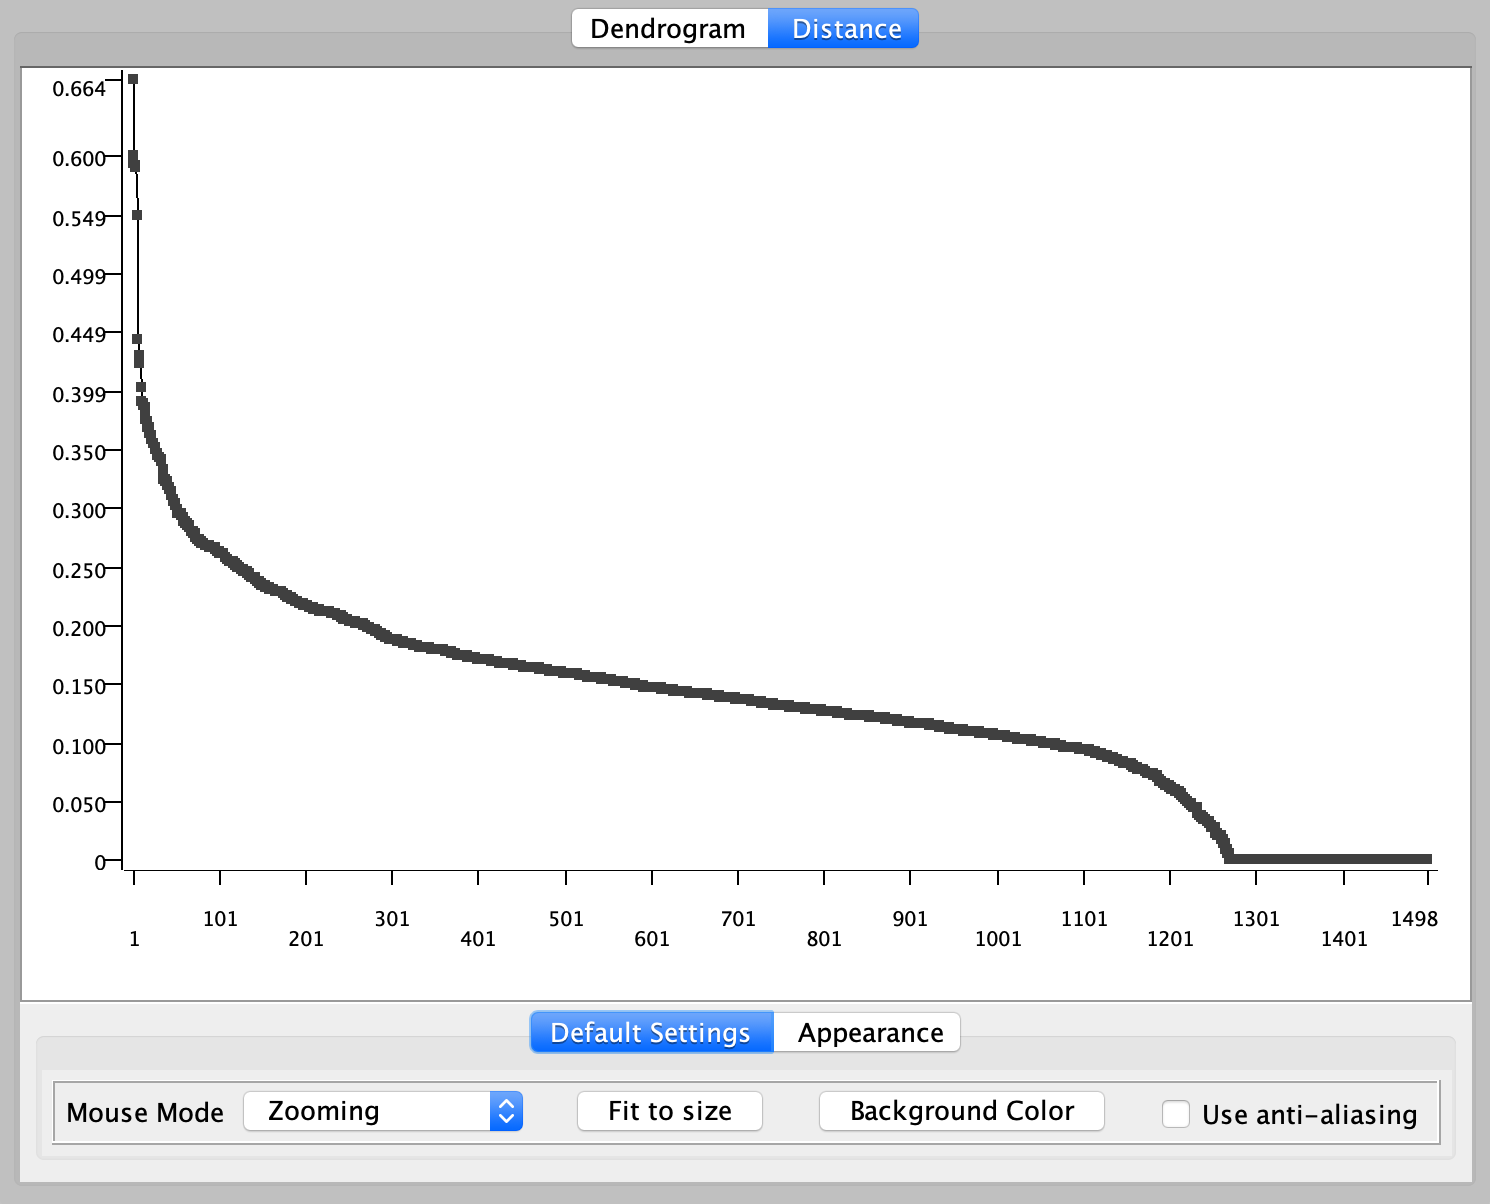
\includegraphics[scale=0.3]{Images/T7_b.png}
    \caption{Visualização da distância}
\end{figure}

\end{document}
